\chapter{Hasil dan Pembahasan}

Bab ini menyajikan hasil penelitian beserta pembahasannya, disusun mengikuti urutan tujuan 
penelitian. Subbab \ref{sec:hasil_dataset} memaparkan hasil pembentukan dataset sebagai 
capaian tujuan pertama. Subbab \ref{sec:hasil_banding} hingga \ref{sec:hasil_perkelas} 
menjawab tujuan kedua melalui perbandingan delapan varian model, analisis kurva evaluasi, 
dan analisis performa per kelas. Subbab \ref{sec:hasil_penyetelan} dan 
\ref{sec:hasil_penyetelan_perkelas} melaporkan hasil optimasi model terpilih melalui 
penyetelan resolusi. Subbab \ref{sec:hasil_sistem} menjawab tujuan ketiga melalui hasil 
implementasi dan pengujian sistem pemantauan, dan Subbab \ref{sec:diskusi_temuan} menutup 
bab ini dengan sintesis temuan lintas subbab.

\section{Hasil Pembentukan Dataset}
\label{sec:hasil_dataset}

Tujuan pertama, yaitu membentuk dataset deteksi objek untuk sembilan kelas khas kawasan 
Malioboro, tercapai melalui proses pengumpulan, pelabelan, dan pembersihan yang diuraikan 
pada Bab III. Dataset akhir memuat 1.581 citra yang terbagi ke dalam himpunan latih, 
validasi, dan uji, dengan distribusi jumlah \textit{instance} tiap kelas sebagaimana telah 
disajikan pada Tabel \ref{tab:distribusi_kelas}. Sebaran spasial dan komposisi kelas pada 
himpunan latih divisualisasikan pada Gambar \ref{fig:labels}, yang memperlihatkan dua 
karakter penting dataset ini.

\begin{figure}[htbp]
    \centering
    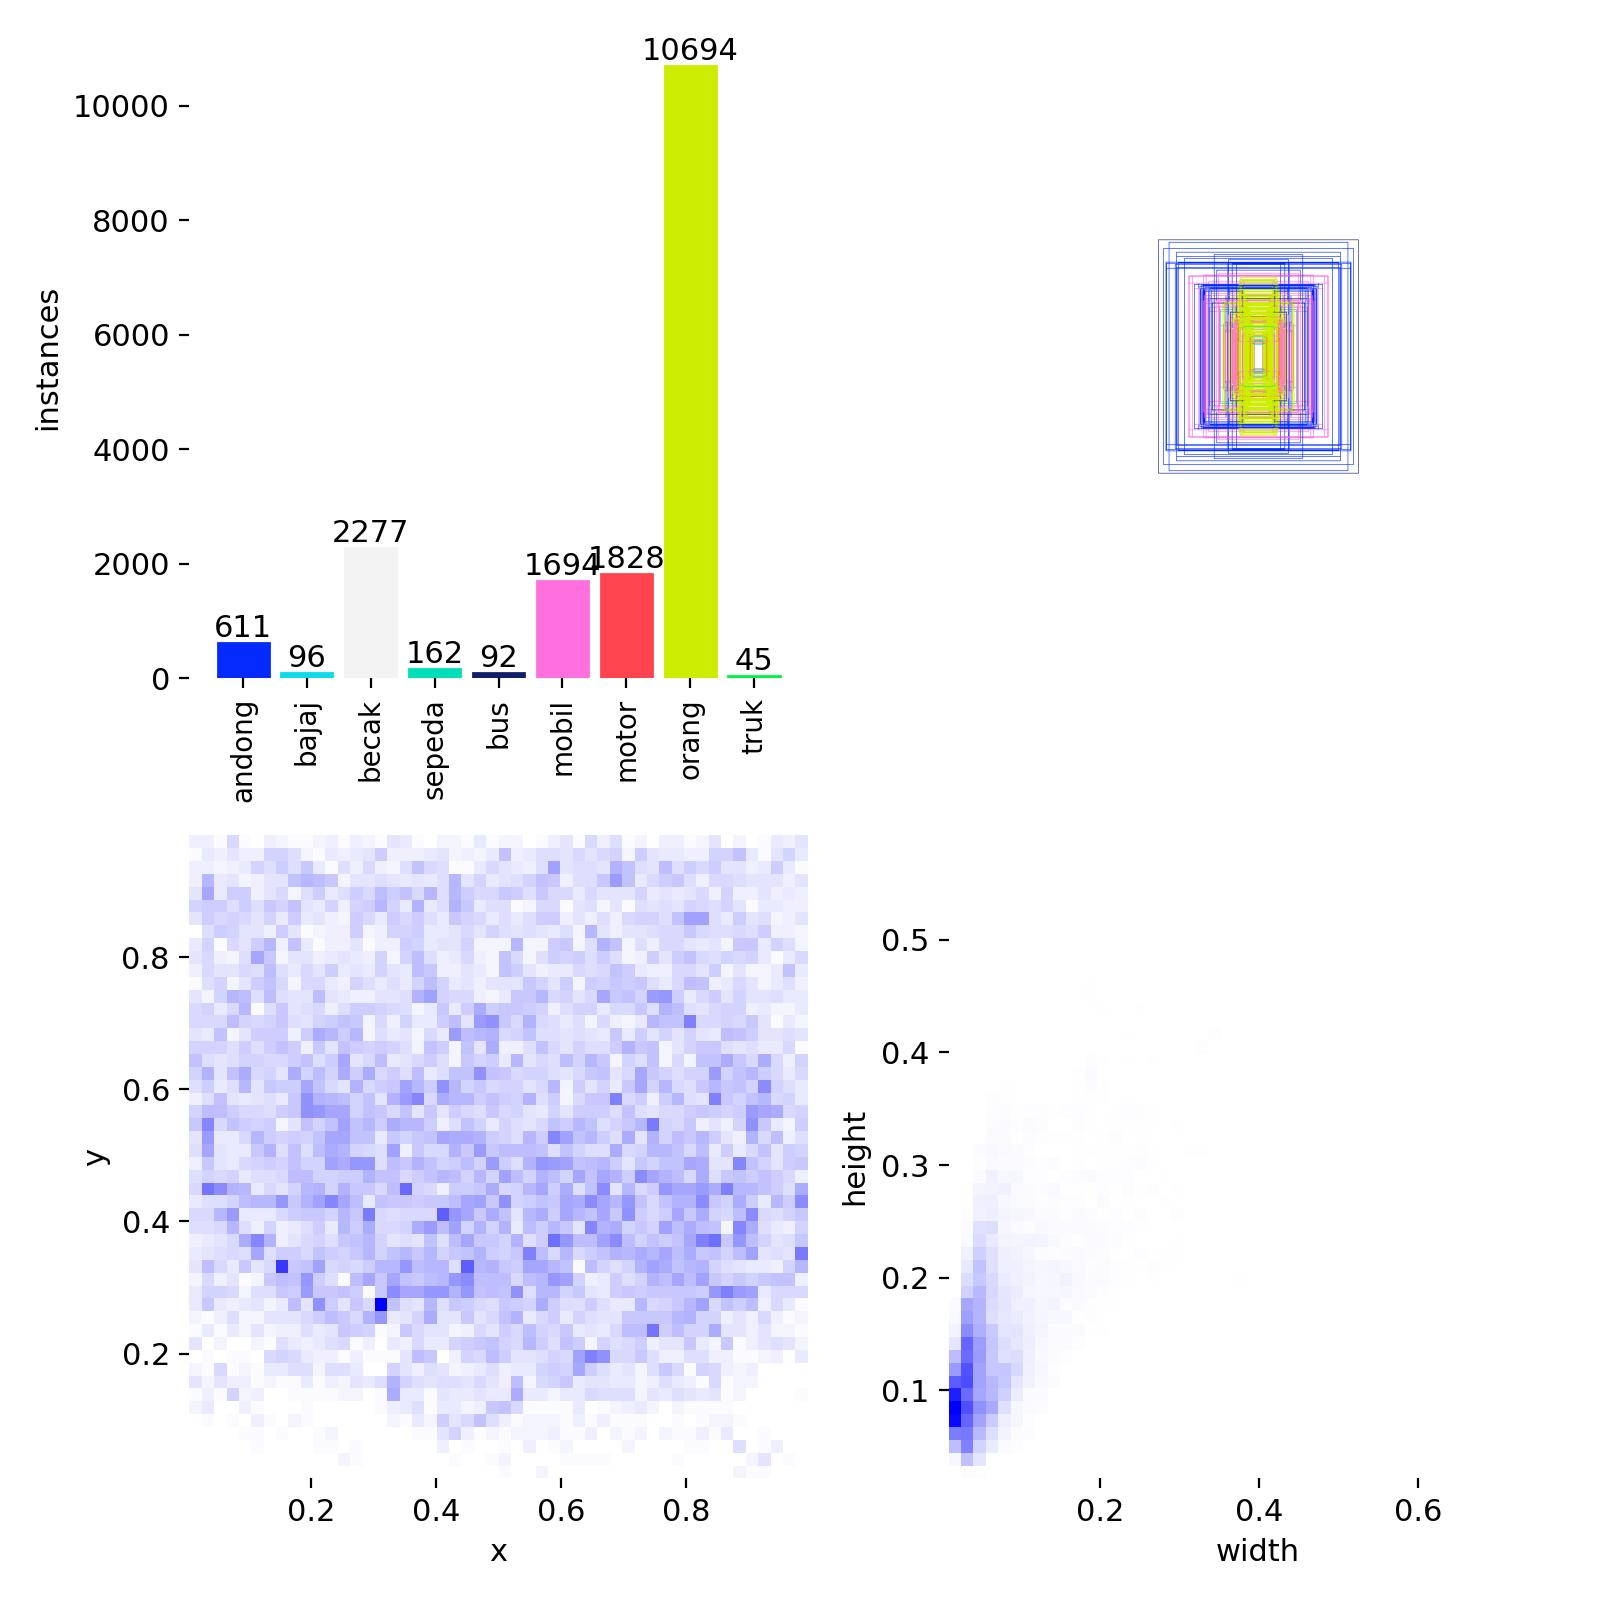
\includegraphics[width=0.9\textwidth]{contents/chapter-4/labels.jpg}
    \caption{Distribusi jumlah \textit{instance} tiap kelas (kiri atas) serta sebaran posisi dan ukuran kotak pembatas pada himpunan latih.}
    \label{fig:labels}
\end{figure}

Karakter pertama adalah ketidakseimbangan kelas yang tajam, terlihat dari dominasi kelas 
orang dengan 10.694 \textit{instance} dibanding kelas truk yang hanya 45 \textit{instance}, 
yaitu rasio sekitar 237 berbanding 1. Karakter kedua adalah dominasi objek berukuran kecil, 
yang tampak pada panel sebaran lebar dan tinggi kotak di Gambar \ref{fig:labels}, dengan 
mayoritas kotak terpusat pada tinggi sekitar 0,1 dari tinggi citra. Kedua karakter ini 
menjadi tantangan utama yang tecermin pada hasil per kelas pada Subbab 
\ref{sec:hasil_perkelas}, dan menjadi dasar strategi penyetelan resolusi pada Subbab 
\ref{sec:hasil_penyetelan}.

\section{Hasil Pelatihan dan Perbandingan Delapan Varian}
\label{sec:hasil_banding}

Delapan varian model, yaitu YOLOv8 dan YOLO11 pada empat ukuran (\textit{nano}, 
\textit{small}, \textit{medium}, \textit{large}), dilatih dengan konfigurasi identik 
sebagaimana diuraikan pada Subbab \ref{sec:pelatihan}, lalu dievaluasi pada himpunan uji 
yang tidak pernah dilihat selama pelatihan. Perbandingan kedelapan varian ini menjadi 
langkah pertama untuk menjawab tujuan kedua penelitian, yaitu menentukan model deteksi yang 
paling sesuai untuk diterapkan pada sistem pemantauan. Subbab ini membandingkan performa 
akurasi dan efisiensi kedelapan varian secara berurutan, sebelum keduanya disandingkan 
sebagai dasar pemilihan model pada Subbab \ref{sec:pemilihan_model}.

\subsection{Perbandingan Akurasi}
\label{sec:perbandingan_akurasi}

Tabel \ref{tab:banding_akurasi} merangkum performa akurasi kedelapan varian pada himpunan 
uji, diurutkan menurun berdasarkan mAP50-95 sebagai metrik lokalisasi yang paling ketat. 
Seluruh nilai pada tabel ini dihitung pada himpunan uji agar perbandingan antar varian 
mencerminkan kemampuan generalisasi yang sesungguhnya, sedangkan himpunan validasi hanya 
digunakan selama pelatihan untuk \textit{early stopping} dan tidak dipakai sebagai dasar 
perbandingan akhir. Susunan tabel dari mAP50-95 tertinggi ke terendah dipilih karena metrik 
ini paling ketat dalam menilai kualitas lokalisasi kotak pembatas, sehingga urutan ini 
menjadi acuan utama pembahasan pada subbab ini.

\begin{table}[htbp]
    \centering
    \caption{Perbandingan akurasi delapan varian model pada himpunan uji.}
    \label{tab:banding_akurasi}
    \begin{tabular}{lccccc}
        \hline
        \textbf{Model} & \textbf{mAP50} & \textbf{mAP50-95} & \textbf{Precision} & \textbf{Recall} & \textbf{Rerata F1} \\
        \hline \hline
        yolo11l & 0,6062 & \textbf{0,4012} & 0,7146 & 0,5438 & 0,5962 \\
        yolov8l & \textbf{0,6175} & 0,3965 & \textbf{0,8355} & 0,5084 & \textbf{0,6222} \\
        yolo11m & 0,6073 & 0,3861 & 0,7559 & 0,5227 & 0,6024 \\
        yolov8m & 0,5875 & 0,3817 & 0,6341 & \textbf{0,5536} & 0,5796 \\
        yolov8s & 0,5845 & 0,3730 & 0,6392 & 0,5247 & 0,5677 \\
        yolo11s & 0,5717 & 0,3646 & 0,7114 & 0,4639 & 0,5488 \\
        yolov8n & 0,5067 & 0,3122 & 0,5472 & 0,5193 & 0,5219 \\
        yolo11n & 0,4698 & 0,2941 & 0,6039 & 0,4234 & 0,4877 \\
        \hline
    \end{tabular}
\end{table}

Performa meningkat seiring bertambahnya ukuran model pada kedua keluarga, dengan varian 
\textit{nano} menempati posisi terbawah dan varian \textit{large} di posisi teratas. Tidak 
ada satu varian yang unggul pada seluruh metrik sekaligus. yolov8l mencapai mAP50 dan 
rerata F1 tertinggi, yaitu 0,6175 dan 0,6222, sedangkan yolo11l mencapai mAP50-95 tertinggi, 
yaitu 0,4012, yang berarti kotak prediksinya rata-rata paling presisi pada berbagai ambang 
IoU. Perbedaan antara dua varian \textit{large} ini tergolong kecil pada akurasi, sehingga 
pertimbangan efisiensi turut menentukan pemilihan akhir.

\subsection{Perbandingan Efisiensi Pelatihan dan Kecepatan Inferensi}
\label{sec:perbandingan_efisiensi}

Tabel \ref{tab:banding_efisiensi} merangkum sisi efisiensi tiap varian, mencakup jumlah 
epoch hingga konvergen, waktu pelatihan, ukuran model, serta kecepatan inferensi. Kecepatan 
pada tabel ini diukur pada GPU Tesla V100-SXM2 di lingkungan pelatihan, sehingga mewakili 
perbandingan relatif antar varian, bukan kecepatan pada perangkat penerapan yang dibahas 
pada Subbab \ref{sec:hasil_sistem}. Jumlah epoch bervariasi karena \textit{early stopping} 
menghentikan pelatihan saat performa validasi berhenti membaik.

\begin{table}[htbp]
    \centering
    \caption{Perbandingan efisiensi delapan varian model. Kecepatan diukur pada GPU Tesla V100.}
    \label{tab:banding_efisiensi}
    \begin{tabular}{lccccc}
        \hline
        \textbf{Model} & \textbf{Epoch} & \textbf{Waktu latih} & \textbf{Ukuran} & \textbf{Waktu inferensi} & \textbf{FPS} \\
         & \textbf{terlatih} & \textbf{(menit)} & \textbf{(MB)} & \textbf{(ms/citra)} & \textbf{(V100)} \\
        \hline \hline
        yolo11l & 74 & 34,9 & 51,20 & 23,10 & 43,3 \\
        yolov8l & 52 & 25,9 & 87,65 & 16,06 & 62,3 \\
        yolo11m & 42 & 14,5 & 40,52 & 15,93 & 62,8 \\
        yolov8m & 64 & 20,1 & 52,03 & 12,33 & 81,1 \\
        yolov8s & 53 & 8,9 & 22,51 & 10,21 & 97,9 \\
        yolo11s & 46 & 8,4 & 19,17 & 13,00 & 76,9 \\
        yolov8n & 100 & 11,2 & 6,25 & 10,45 & 95,7 \\
        yolo11n & 91 & 11,1 & 5,47 & 12,98 & 77,0 \\
        \hline
    \end{tabular}
\end{table}

Gambar \ref{fig:konvergensi} membandingkan pola konvergensi dua varian \textit{large} 
sepanjang pelatihan, diplot dari nilai mAP50-95 pada data validasi tiap epoch. Kedua model 
menunjukkan kenaikan tajam pada epoch-epoch awal yang kemudian disusul fluktuasi di sekitar 
nilai yang relatif stabil, menandakan model telah memanfaatkan sebagian besar kapasitas 
belajarnya. yolo11l berhenti pada epoch ke-74 dengan mAP50-95 validasi akhir di kisaran 
0,38, sedikit di atas yolov8l yang berhenti pada epoch ke-52 dengan nilai akhir di kisaran 
0,35, konsisten dengan keunggulan yolo11l pada metrik ini di Tabel \ref{tab:banding_akurasi}.

\begin{figure}[htbp]
    \centering
    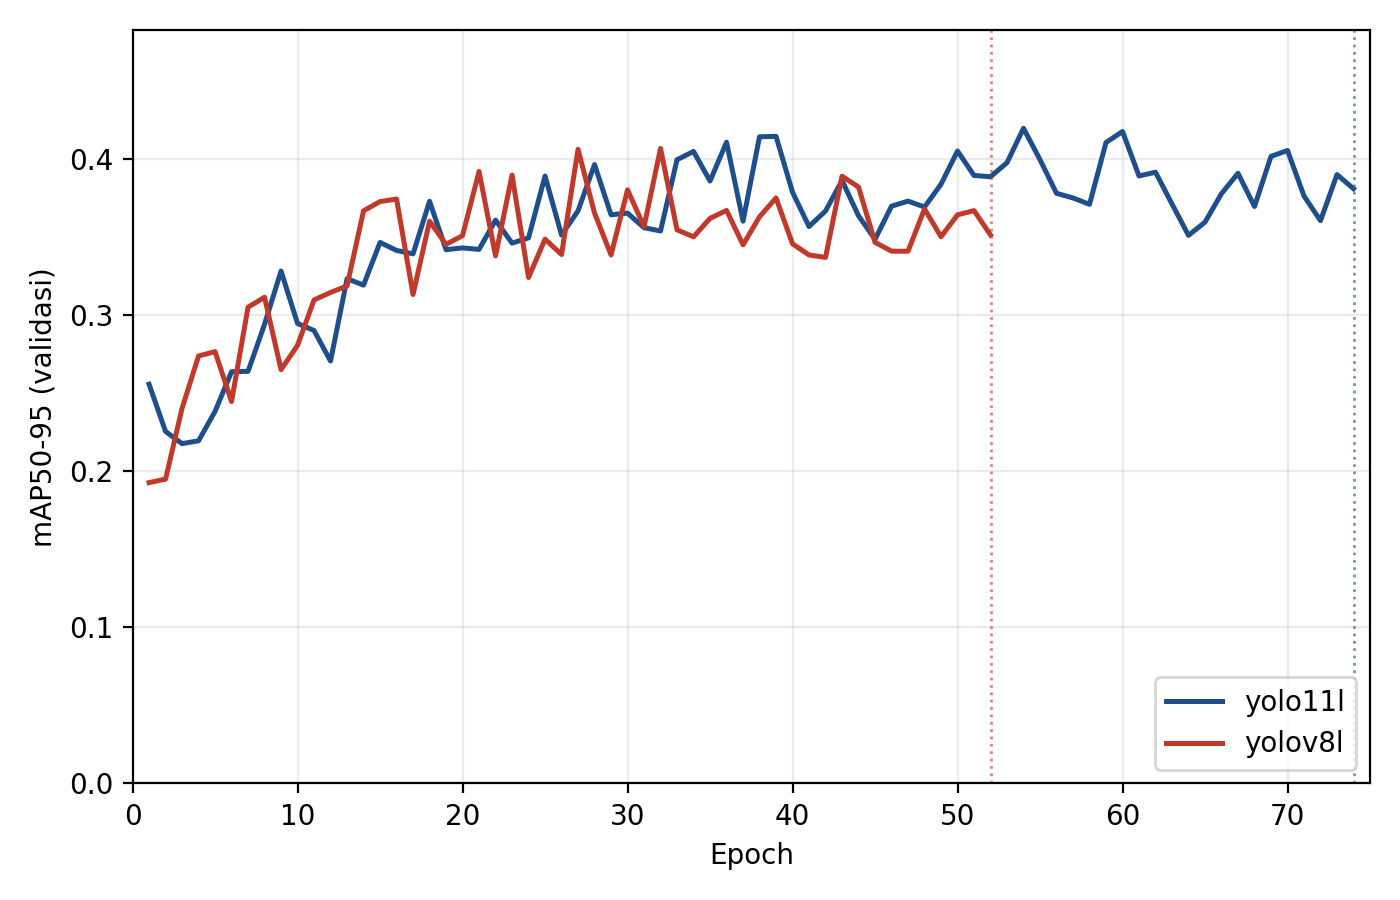
\includegraphics[width=0.85\textwidth]{contents/chapter-4/konvergensi.png}
    \caption{Perkembangan mAP50-95 pada data validasi sepanjang epoch untuk yolo11l dan yolov8l.}
    \label{fig:konvergensi}
\end{figure}

\subsection{Pemilihan Model Terbaik}
\label{sec:pemilihan_model}

Hasil pada Tabel \ref{tab:banding_akurasi} dan \ref{tab:banding_efisiensi} menunjukkan tidak 
ada satu varian yang unggul pada seluruh metrik sekaligus, sehingga pemilihan model terbaik 
memerlukan pertimbangan yang menyeimbangkan akurasi, ukuran, dan kecepatan, bukan sekadar 
memilih nilai tertinggi pada satu kolom. Subbab ini menjelaskan pertimbangan tersebut secara 
eksplisit, dengan menyandingkan dua kandidat utama, yaitu yolo11l dan yolov8l, sebagai dua 
varian \textit{large} yang sama-sama unggul dibanding varian lain pada keluarganya. 
Pemilihan ini dibuat secara jujur dengan menyadari yolov8l sedikit unggul pada mAP50 dan 
rerata F1 serta lebih cepat pada GPU V100, sehingga keputusan akhirnya tidak didasarkan pada 
satu keunggulan mutlak melainkan pada akumulasi beberapa pertimbangan yang saling melengkapi.

Pertimbangan pertama adalah lokalisasi. yolo11l unggul pada mAP50-95, yaitu metrik yang 
menuntut kotak pembatas presisi pada berbagai ambang IoU, yang menandakan lokalisasi 
objeknya lebih rapi dibanding yolov8l meski selisih mAP50 keduanya tipis. Pertimbangan 
kedua adalah ukuran model, yang menjadi penentu untuk perangkat penerapan dengan memori GPU 
terbatas. Ukuran yolo11l hanya 51,20 MB dibanding 87,65 MB milik yolov8l, yaitu sekitar 42\% 
lebih ringkas, sehingga menyisakan ruang memori yang lebih lega untuk pemrosesan 
\textit{stream} dan beban sistem lainnya pada laptop dengan GPU GTX 1650 bermemori 4 GB.

Pertimbangan ketiga muncul dari pengujian kecepatan inferensi pada perangkat penerapan 
sesungguhnya, yang justru membalikkan urutan pada GPU V100. Pada Subbab 
\ref{sec:kecepatan_gtx} ditunjukkan bahwa pada GTX 1650, yolo11l mencapai 9,73 FPS, lebih 
cepat dibanding yolov8l yang hanya 8,80 FPS, berkebalikan dengan hasil pada GPU V100 saat 
yolov8l lebih cepat. Atas dasar ketiga pertimbangan ini, yaitu lokalisasi yang lebih presisi, 
ukuran yang lebih ringkas, dan kecepatan yang ternyata lebih unggul pada perangkat target, 
yolo11l dipilih sebagai model yang diterapkan pada sistem. Pilihan ini kemudian diperkuat 
oleh hasil penyetelan pada Subbab \ref{sec:hasil_penyetelan}, yang menunjukkan rerata F1 
yolo11l naik menjadi 0,6739 setelah optimasi resolusi, melampaui capaian seluruh varian pada 
resolusi dasar termasuk yolov8l.

\section{Analisis Kurva Evaluasi Model Terpilih}
\label{sec:analisis_kurva}

Selain metrik tunggal pada Tabel \ref{tab:banding_akurasi}, perilaku model terpilih yolo11l 
pada berbagai ambang keyakinan dapat ditelaah melalui kurva evaluasi yang dihasilkan 
Ultralytics. Kurva \textit{precision-recall} dan kurva F1 pada Gambar 
\ref{fig:pr_curve_yolo11l} dan \ref{fig:f1_curve_yolo11l} dihasilkan dari evaluasi otomatis 
pada himpunan validasi di akhir pelatihan, dan digunakan di sini untuk menelaah perilaku 
model pada berbagai ambang keyakinan serta menentukan titik operasi yang dipakai pada 
sistem. Hasil akhir model, yaitu performa pada data yang sama sekali tidak dilihat selama 
pelatihan, tetap diukur tersendiri pada himpunan uji dan disajikan melalui 
\textit{confusion matrix} ternormalisasi pada Gambar \ref{fig:confusion_matrix} serta 
metrik per kelas pada Subbab \ref{sec:hasil_perkelas}.

\begin{figure}[htbp]
    \centering
    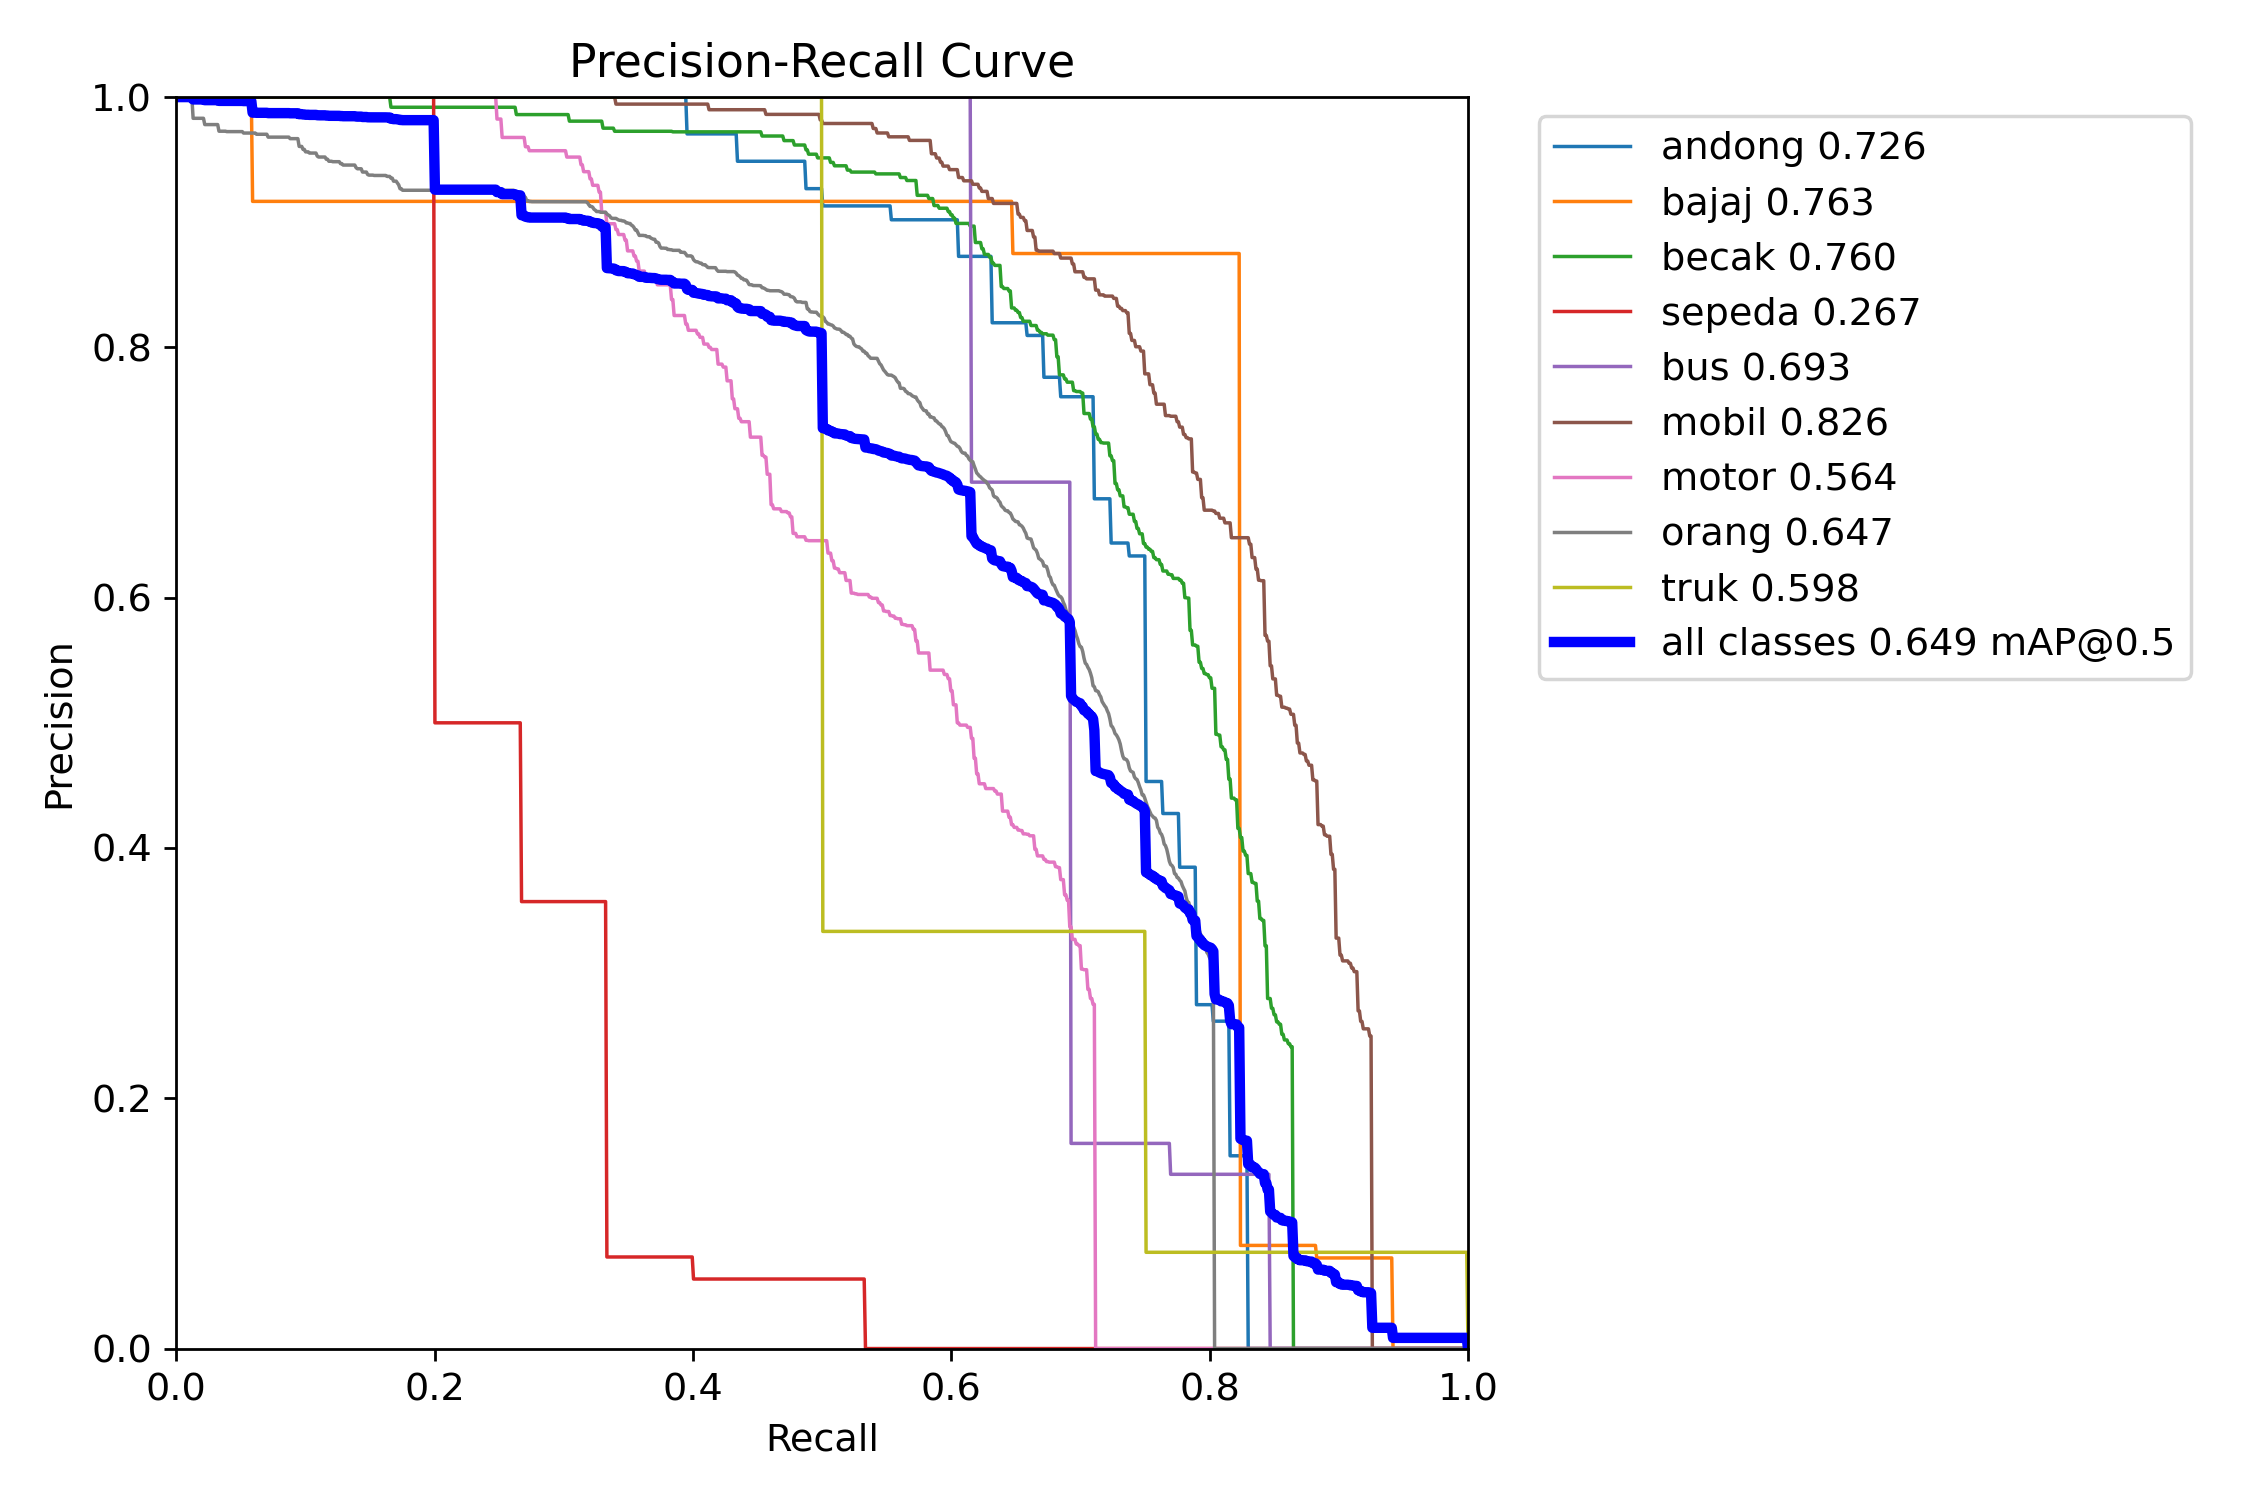
\includegraphics[width=0.75\textwidth]{contents/chapter-4/yolo11l_PR_curve.png}
    \caption{Kurva \textit{precision-recall} model yolo11l untuk seluruh kelas pada himpunan validasi.}
    \label{fig:pr_curve_yolo11l}
\end{figure}

Gambar \ref{fig:pr_curve_yolo11l} menunjukkan kurva \textit{precision-recall} tiap kelas 
pada himpunan validasi. Kelas dengan kurva yang menjorok ke kanan atas, seperti mobil dan 
andong, mempertahankan \textit{precision} tinggi hingga \textit{recall} yang juga tinggi, 
menandakan model mengenali kelas tersebut dengan keyakinan yang konsisten. Sebaliknya, 
kelas seperti sepeda menunjukkan kurva yang jatuh tajam segera setelah \textit{recall} 
kecil, menandakan model hanya mampu mengenali sebagian kecil objek sepeda sebelum 
\textit{precision}-nya merosot. Pola ini sejalan dengan hasil pada himpunan uji yang dibahas 
pada Subbab \ref{sec:hasil_perkelas}, meski kedua himpunan berbeda.

\begin{figure}[htbp]
    \centering
    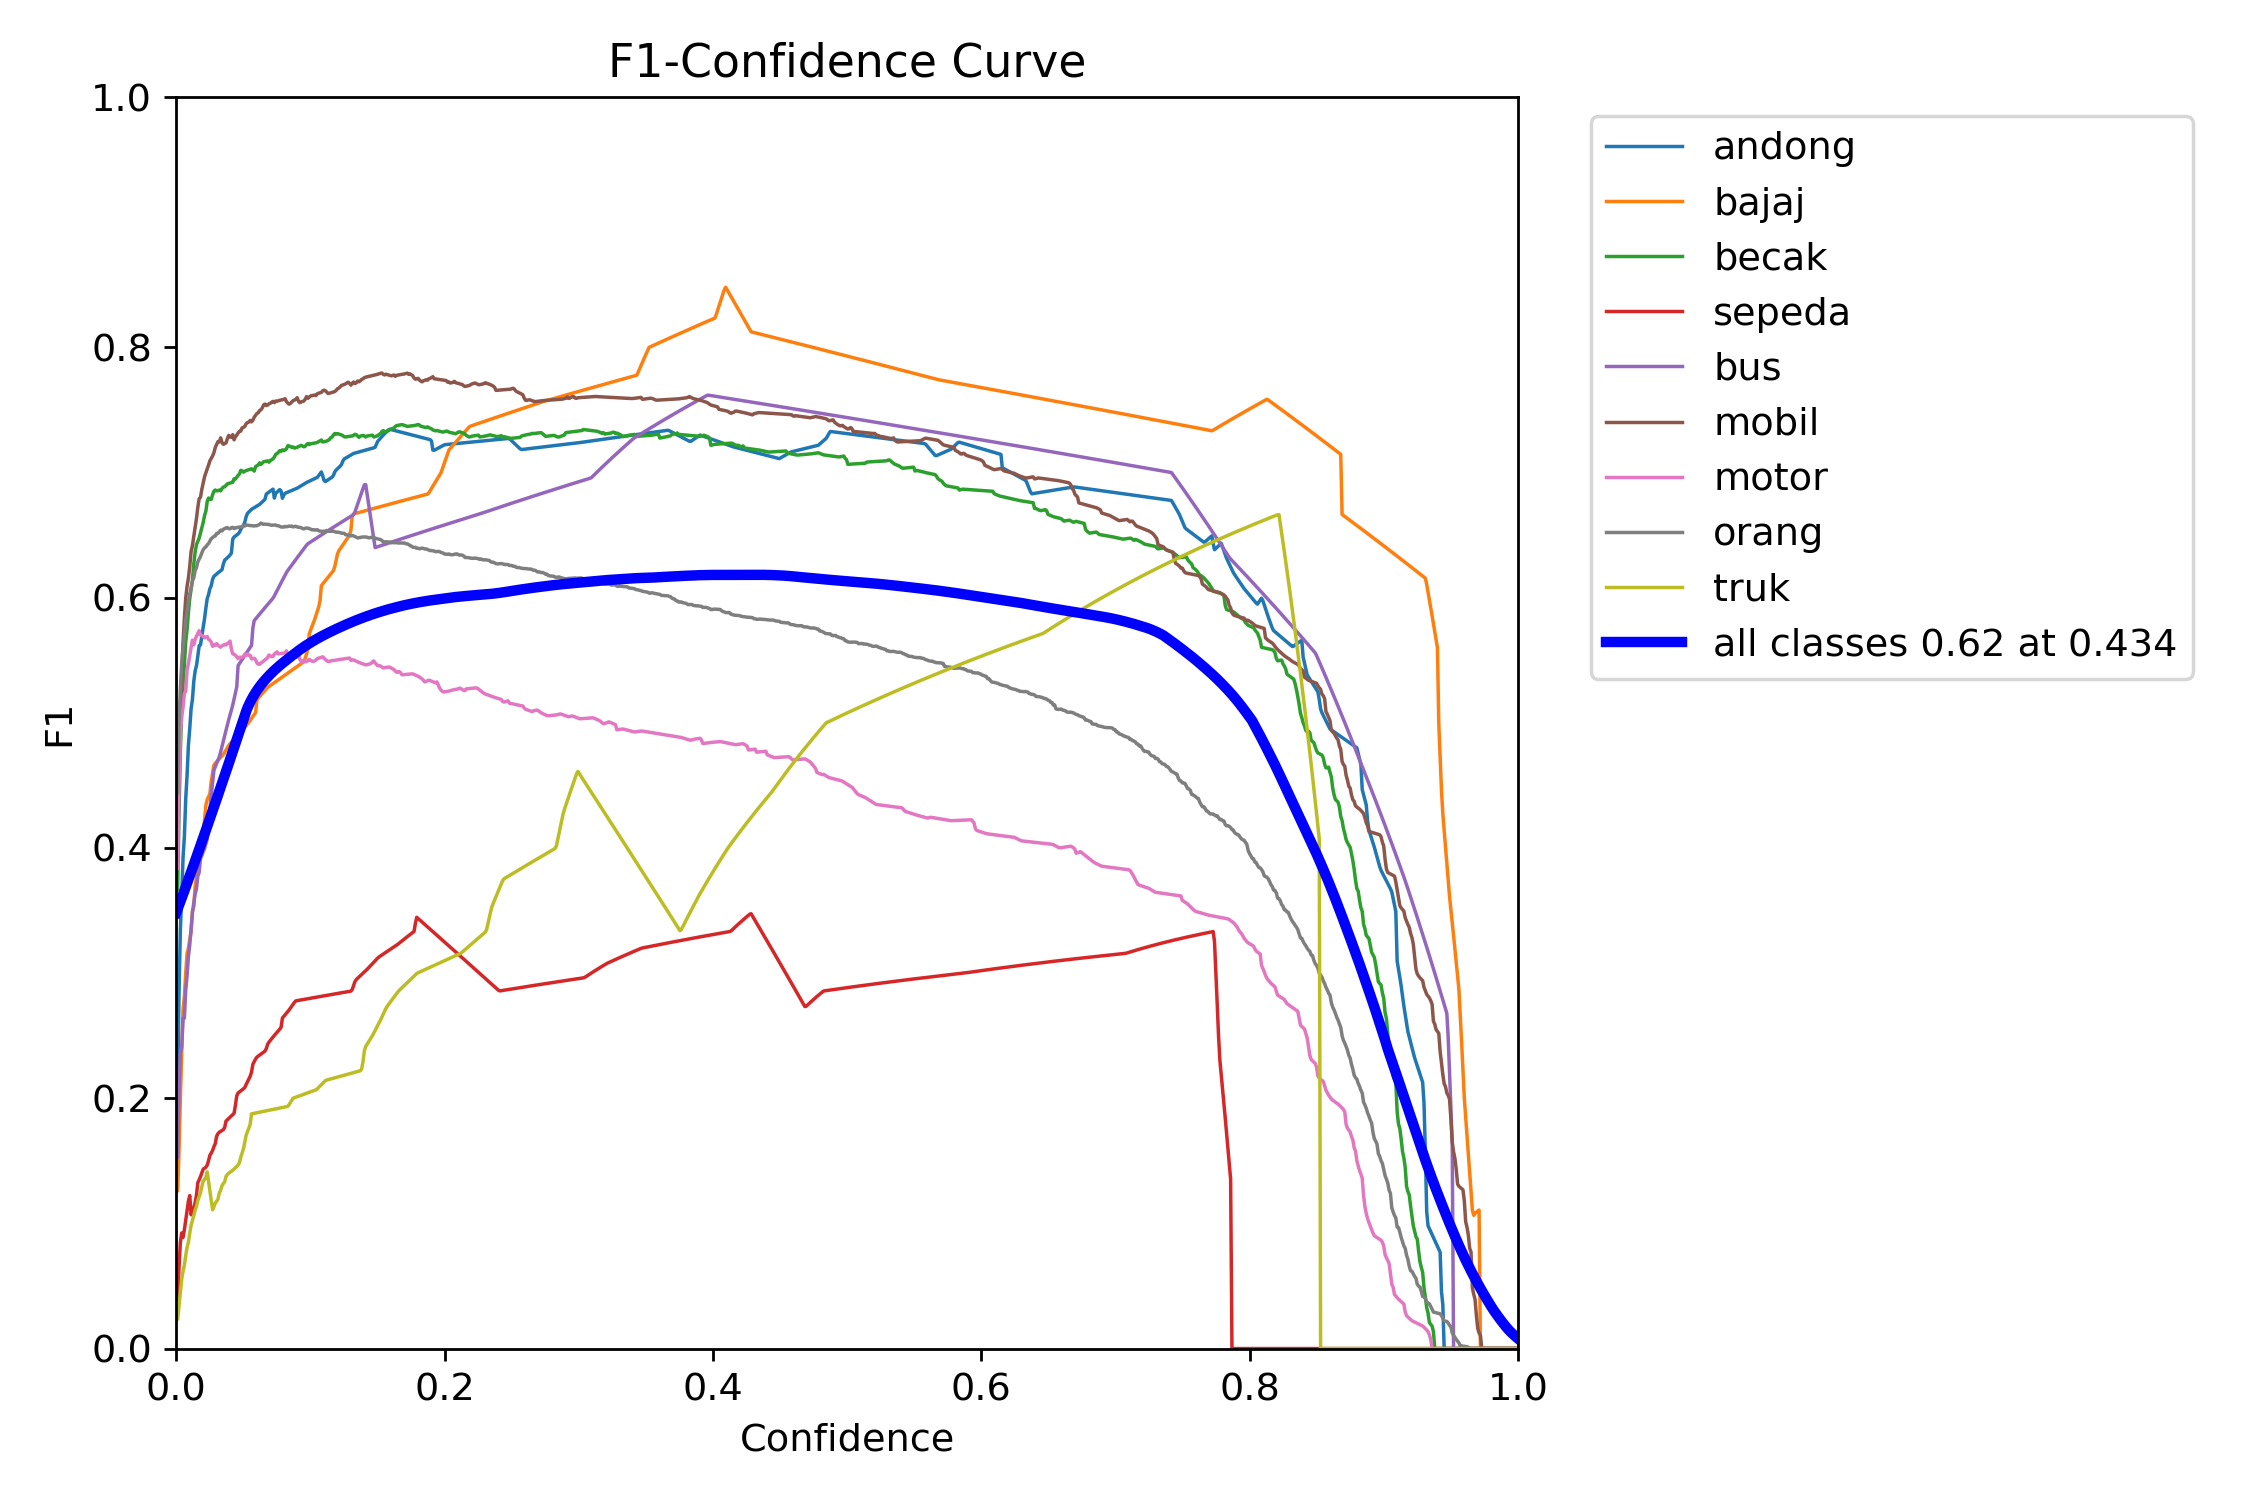
\includegraphics[width=0.75\textwidth]{contents/chapter-4/yolo11l_F1_curve.png}
    \caption{Kurva F1-\textit{score} terhadap ambang keyakinan model yolo11l untuk seluruh kelas pada himpunan validasi.}
    \label{fig:f1_curve_yolo11l}
\end{figure}

Gambar \ref{fig:f1_curve_yolo11l} memperlihatkan F1 pada himpunan validasi sebagai fungsi 
ambang keyakinan, yang berguna untuk menentukan titik operasi model. Puncak kurva rerata 
seluruh kelas menunjukkan ambang keyakinan yang mengoptimalkan F1 secara keseluruhan, dan 
ambang inilah yang dipakai sebagai titik operasi pada sistem yang diterapkan. Lebar puncak 
yang relatif landai menandakan performa model tidak terlalu sensitif terhadap pemilihan 
ambang di sekitar titik optimalnya, sehingga sistem tetap stabil meski ambang digeser 
sedikit untuk menyesuaikan kebutuhan operasional. Metrik akhir yang dilaporkan pada Tabel 
\ref{tab:perkelas} tetap dihitung pada himpunan uji menggunakan ambang ini, bukan diambil 
langsung dari kurva validasi.

\begin{figure}[htbp]
    \centering
    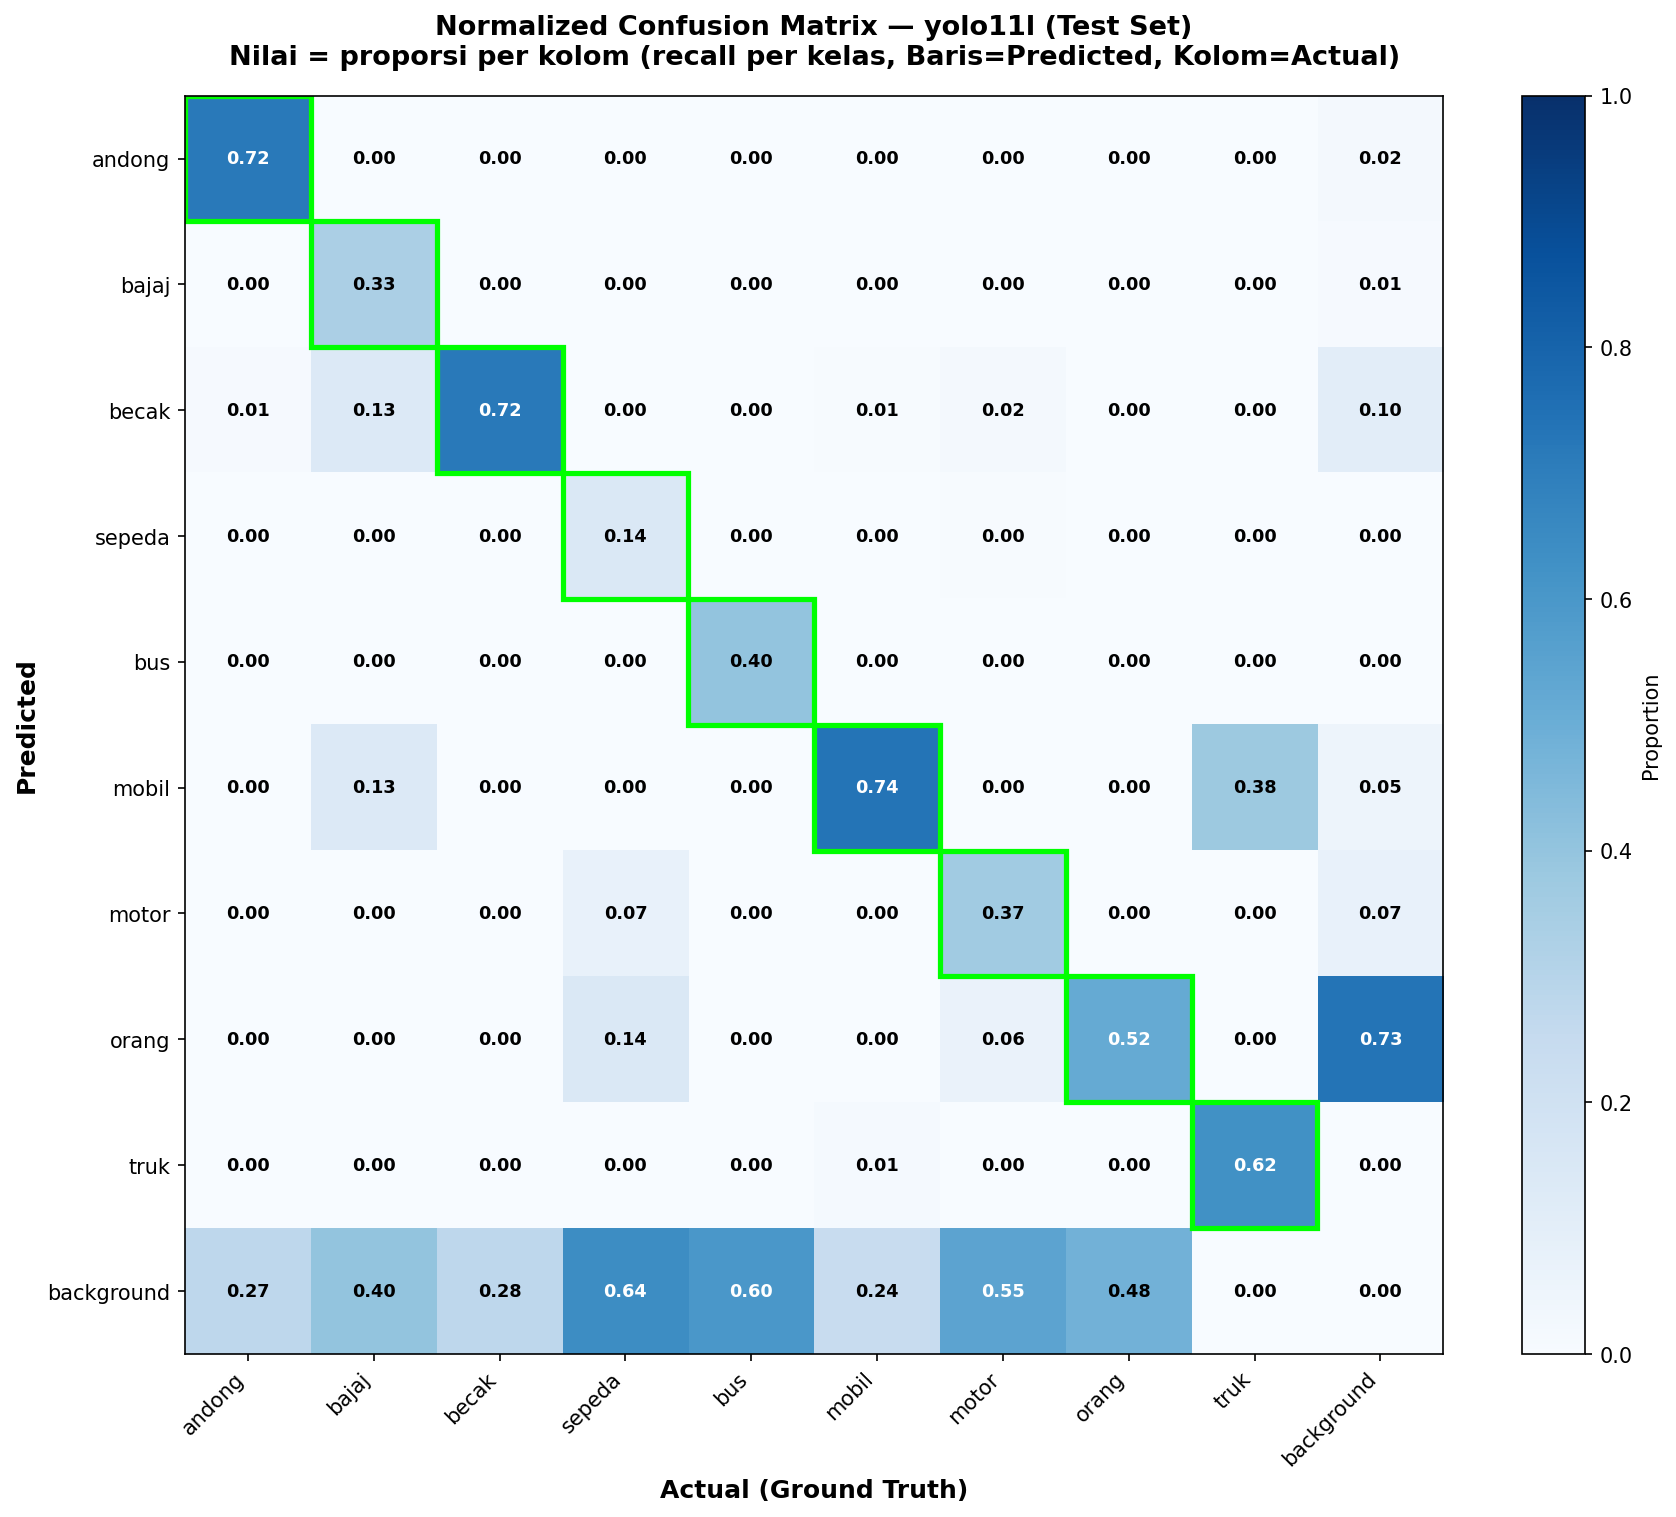
\includegraphics[width=0.8\textwidth]{contents/chapter-4/yolo11l_confusion_matrix_normalized.png}
    \caption{\textit{Confusion matrix} ternormalisasi model yolo11l pada himpunan uji.}
    \label{fig:confusion_matrix}
\end{figure}

\textit{Confusion matrix} ternormalisasi pada Gambar \ref{fig:confusion_matrix} memetakan ke 
kelas apa suatu objek paling sering salah diklasifikasikan, atau apakah ia gagal terdeteksi 
sama sekali (kolom \textit{background}). Diagonal utama yang gelap pada kelas mobil, andong, 
dan becak menegaskan deteksi yang andal pada kelas-kelas tersebut. Sebaliknya, baris kelas 
sepeda dan motor menunjukkan proporsi besar yang jatuh ke kolom \textit{background}, berarti 
kesalahan dominan pada kedua kelas ini adalah objek yang gagal terdeteksi, bukan tertukar 
ke kelas lain. Pengamatan ini konsisten dengan pola \textit{recall} rendah yang dibahas 
lebih rinci pada Subbab \ref{sec:hasil_perkelas}.

\section{Analisis Performa per Kelas dan Pengaruh Ketidakseimbangan}
\label{sec:hasil_perkelas}

Performa keseluruhan dan kurva evaluasi pada subbab sebelumnya belum cukup menggambarkan 
perilaku model pada tiap kelas, terutama pada dataset yang timpang seperti ini. Gambar 
\ref{fig:f1_heatmap} memetakan F1 tiap kelas untuk kedelapan varian, dan memperlihatkan pola 
yang konsisten lintas model, yaitu beberapa kelas selalu mudah dideteksi sementara kelas 
lain selalu sulit. Tabel \ref{tab:perkelas} merinci performa per kelas untuk model terpilih 
yolo11l, disandingkan dengan jumlah \textit{instance} latih tiap kelas agar pengaruh 
ketidakseimbangan dapat ditelaah.

\begin{figure}[htbp]
    \centering
    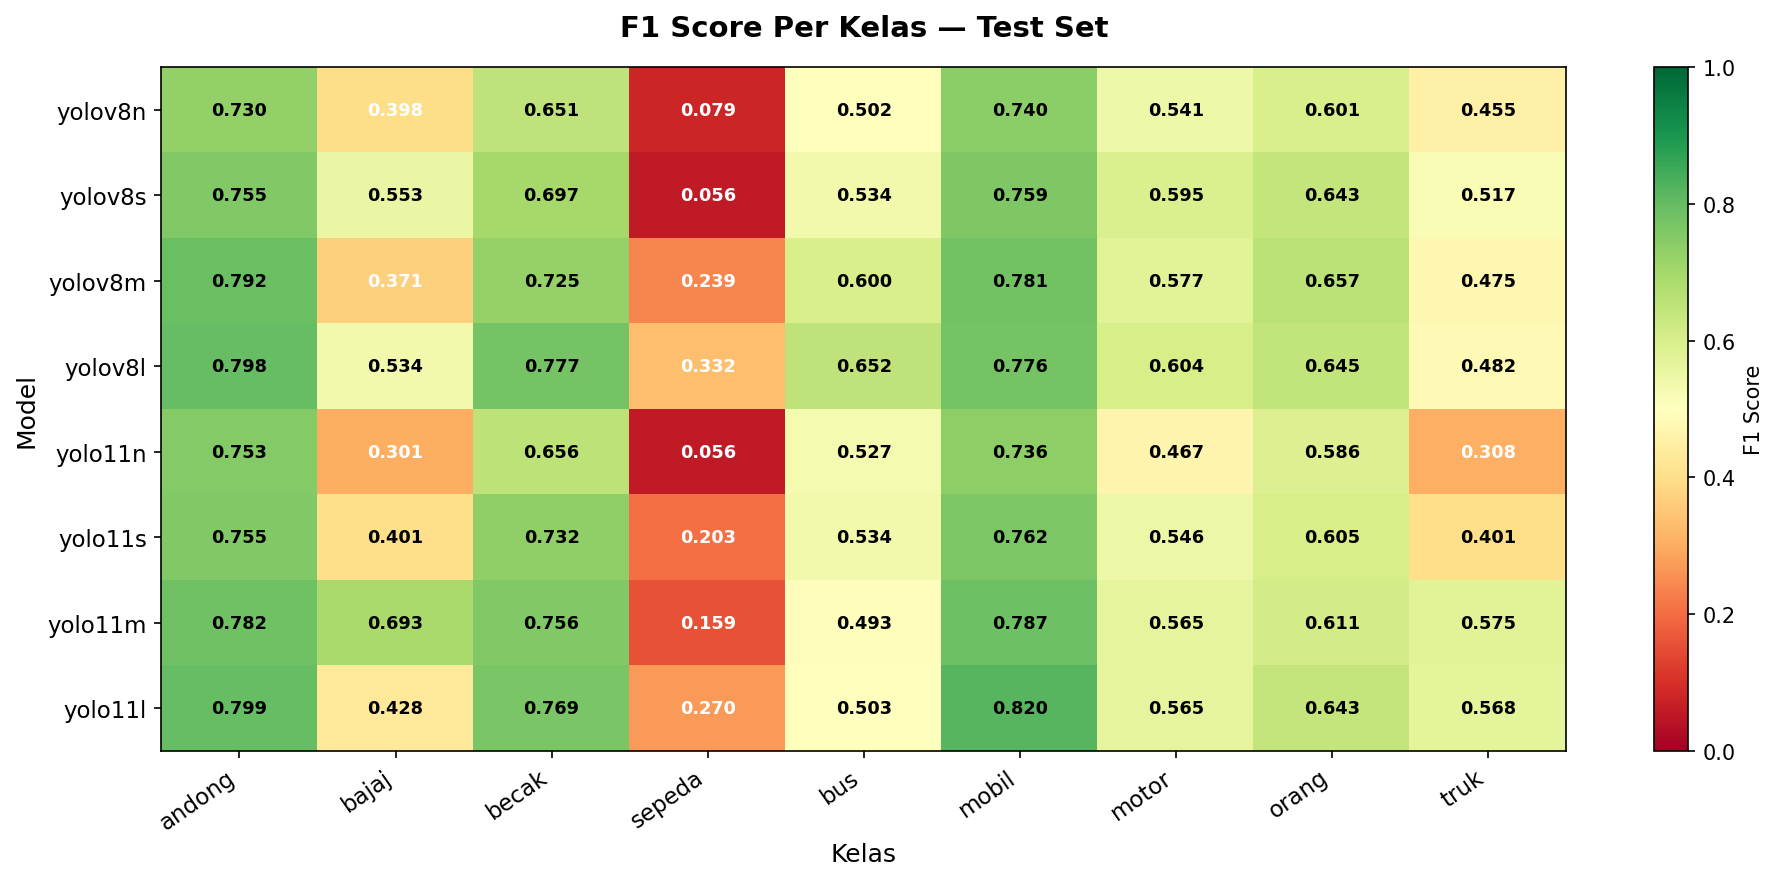
\includegraphics[width=\textwidth]{contents/chapter-4/f1_heatmap.png}
    \caption{F1 per kelas pada himpunan uji untuk kedelapan varian model.}
    \label{fig:f1_heatmap}
\end{figure}

\begin{table}[htbp]
    \centering
    \caption{Performa per kelas model terpilih yolo11l pada himpunan uji, disandingkan jumlah \textit{instance} latih.}
    \label{tab:perkelas}
    \begin{tabular}{lcccc}
        \hline
        \textbf{Kelas} & \textbf{Instans latih} & \textbf{Precision} & \textbf{Recall} & \textbf{F1} \\
        \hline \hline
        mobil & 1.694 & 0,889 & 0,761 & 0,820 \\
        andong & 611 & 0,889 & 0,726 & 0,799 \\
        becak & 2.277 & 0,816 & 0,727 & 0,769 \\
        orang & 10.694 & 0,804 & 0,536 & 0,643 \\
        truk & 45 & 0,458 & 0,750 & 0,568 \\
        motor & 1.828 & 0,886 & 0,415 & 0,565 \\
        bus & 92 & 0,678 & 0,400 & 0,503 \\
        bajaj & 96 & 0,460 & 0,400 & 0,428 \\
        sepeda & 162 & 0,553 & 0,179 & 0,270 \\
        \hline
    \end{tabular}
\end{table}

Pola yang paling menonjol adalah rendahnya \textit{recall} pada banyak kelas, sejalan dengan 
pengamatan pada \textit{confusion matrix} di Subbab \ref{sec:analisis_kurva}. Kelas motor, 
misalnya, memiliki \textit{precision} 0,886 tetapi \textit{recall} hanya 0,415, dan kelas 
orang memiliki \textit{recall} 0,536 yang berarti hampir separuh objek orang tidak 
terdeteksi. Pola ini menandakan kesalahan dominan model adalah objek yang terlewat, bukan 
deteksi keliru, dan objek yang terlewat umumnya berukuran kecil atau berada jauh dari kamera.

Pengaruh ketidakseimbangan kelas terlihat, tetapi tidak bersifat tunggal. Kelas dengan 
performa terbaik adalah mobil, andong, dan becak dengan F1 di atas 0,76, yaitu kelas yang 
berisi objek berukuran sedang hingga besar dengan bentuk yang khas dan jumlah 
\textit{instance} memadai. Sebaliknya, kelas terlemah adalah sepeda dengan F1 hanya 0,270, 
diikuti bajaj dan bus, yaitu kelas dengan \textit{instance} paling sedikit. Akan tetapi, 
hubungan ini tidak monoton. Kelas truk yang hanya memiliki 45 \textit{instance}, paling 
sedikit di antara semua kelas, justru mencapai F1 0,568 yang melampaui sepeda dengan 162 
\textit{instance}.

Anomali ini menunjukkan bahwa ukuran dan kekhasan visual objek turut menentukan, di samping 
jumlah \textit{instance}. Truk berukuran besar dan berpenampilan khas sehingga lebih mudah 
dipelajari meski contohnya sedikit, sedangkan sepeda berukuran kecil dan mudah tertukar 
dengan motor sehingga tetap sulit dikenali walau contohnya lebih banyak. Dengan demikian, 
ketidakseimbangan kelas adalah faktor yang berpengaruh, tetapi efeknya dimediasi oleh ukuran 
objek dan tingkat kemiripannya dengan kelas lain. Temuan inilah yang mendasari strategi 
penyetelan melalui peningkatan resolusi masukan, yang dibahas pada subbab berikutnya.

\section{Hasil Penyetelan Hyperparameter Model Terpilih}
\label{sec:hasil_penyetelan}

Model terpilih yolo11l dioptimasi lebih lanjut melalui penyetelan resolusi citra masukan 
dari 640 menjadi 960 piksel, dengan dasar dan strategi sebagaimana diuraikan pada Subbab 
\ref{sec:penyetelan}. Penyetelan ini diarahkan secara khusus pada kelemahan yang telah 
teridentifikasi pada Subbab \ref{sec:hasil_perkelas}, yaitu \textit{recall} rendah pada 
objek berukuran kecil, sehingga hasil yang dipaparkan pada subbab ini sekaligus menjadi 
pengujian terhadap hipotesis tersebut. Model hasil penyetelan berhenti pada epoch ke-79 
akibat \textit{early stopping}, sebanding dengan model awal yang berhenti pada epoch ke-74, 
sehingga keduanya sama-sama mencapai konvergensi sebelum batas 100 epoch dan perbandingan 
performa keduanya tetap adil.

Tabel \ref{tab:perbandingan_penyetelan} membandingkan performa keseluruhan pada himpunan 
uji antara konfigurasi resolusi 640 dan 960. Seluruh metrik meningkat setelah resolusi 
dinaikkan, tanpa ada satu pun yang menurun, sebuah hasil yang konsisten dan tidak ambigu 
untuk menilai efektivitas penyetelan ini. Konsistensi kenaikan pada seluruh metrik 
sekaligus, alih-alih kenaikan pada satu metrik dengan kompensasi penurunan pada metrik lain, 
menunjukkan bahwa resolusi yang lebih tinggi memang memperbaiki kualitas deteksi secara 
menyeluruh, bukan sekadar menggeser titik seimbang antara \textit{precision} dan 
\textit{recall}.

\begin{table}[htbp]
    \centering
    \caption{Perbandingan performa yolo11l pada resolusi 640 dan 960 (himpunan uji).}
    \label{tab:perbandingan_penyetelan}
    \begin{tabular}{lccccc}
        \hline
        \textbf{Konfigurasi} & \textbf{mAP50} & \textbf{mAP50-95} & \textbf{Precision} & \textbf{Recall} & \textbf{Rerata F1} \\
        \hline \hline
        Resolusi 640 (awal) & 0,6062 & 0,4012 & 0,7146 & 0,5438 & 0,5962 \\
        Resolusi 960 (setelan) & 0,6497 & 0,4413 & 0,7575 & 0,6217 & 0,6739 \\
        \hline
        Selisih & +0,0435 & +0,0401 & +0,0429 & +0,0779 & +0,0777 \\
        \hline
    \end{tabular}
\end{table}

Nilai mAP50-95 naik 0,0401 atau sekitar empat poin persentase, peningkatan yang besar untuk 
satu perubahan \textit{hyperparameter} tunggal. Kenaikan terbesar terjadi pada 
\textit{recall}, yaitu 0,0779, sesuai hipotesis bahwa resolusi lebih tinggi membuat lebih 
banyak objek kecil berhasil terdeteksi alih-alih terlewat, sebagaimana terlihat dari 
banyaknya kasus FN pada Tabel \ref{tab:perkelas}. Kenaikan \textit{precision} yang menyertai 
\textit{recall}, yaitu sebesar 0,0429, menunjukkan bahwa perbaikan ini tidak diperoleh 
dengan mengorbankan ketelitian deteksi, melainkan model benar-benar mengenali lebih banyak 
objek dengan tingkat kesalahan yang tetap terkendali.

Biaya komputasi turut meningkat sejalan dengan perbaikan akurasi ini. Waktu pelatihan naik 
dari 34,9 menit menjadi 84,2 menit akibat ukuran citra yang lebih besar, sedangkan ukuran 
model praktis tidak berubah pada 51,25 MB karena arsitektur tetap sama. Biaya pelatihan ini 
bersifat sekali jalan dan tidak menjadi beban berulang saat sistem dioperasikan. Pada GPU 
V100, kecepatan inferensi turun dari 23,10 ms (43,3 FPS) pada resolusi 640 menjadi 25,46 ms 
(39,3 FPS) pada resolusi 960, penurunan yang tergolong kecil mengingat kenaikan resolusi 
masukannya, dan masih jauh di atas kebutuhan \textit{real-time}. Kecepatan pada perangkat 
penerapan yang sebenarnya dibahas pada Subbab \ref{sec:hasil_sistem}.

\section{Analisis Performa per Kelas Setelah Penyetelan}
\label{sec:hasil_penyetelan_perkelas}

Kenaikan metrik keseluruhan pada Subbab \ref{sec:hasil_penyetelan} belum menjelaskan kelas 
mana yang paling berkontribusi terhadap perbaikan tersebut, sehingga diperlukan analisis 
yang lebih terperinci pada tingkat kelas. Tabel \ref{tab:f1_penyetelan} merinci perbandingan 
F1 per kelas antara resolusi 640 dan 960, disusun untuk menelaah kelas mana yang paling 
diuntungkan oleh penyetelan resolusi dan kelas mana yang relatif tidak terpengaruh. 
Perbandingan pada tingkat kelas ini juga berfungsi memverifikasi apakah penyetelan benar-
benar menyasar kelemahan yang telah teridentifikasi pada Subbab \ref{sec:hasil_perkelas}, 
yaitu kelas berukuran kecil dengan \textit{recall} rendah.

\begin{table}[htbp]
    \centering
    \caption{Perbandingan F1 per kelas yolo11l pada resolusi 640 dan 960 (himpunan uji).}
    \label{tab:f1_penyetelan}
    \begin{tabular}{lccc}
        \hline
        \textbf{Kelas} & \textbf{F1 (640)} & \textbf{F1 (960)} & \textbf{Selisih} \\
        \hline \hline
        andong & 0,799 & 0,785 & $-$0,014 \\
        bajaj & 0,428 & 0,660 & +0,232 \\
        becak & 0,769 & 0,814 & +0,045 \\
        sepeda & 0,270 & 0,472 & +0,202 \\
        bus & 0,503 & 0,620 & +0,117 \\
        mobil & 0,820 & 0,814 & $-$0,006 \\
        motor & 0,565 & 0,621 & +0,056 \\
        orang & 0,643 & 0,654 & +0,011 \\
        truk & 0,568 & 0,625 & +0,057 \\
        \hline
        Rerata & 0,596 & 0,674 & +0,078 \\
        \hline
    \end{tabular}
\end{table}

Perbaikan paling jelas terlihat pada kelas yang sebelumnya paling lemah. Kelas sepeda naik 
0,202 poin F1, sedangkan kelas bajaj naik 0,232 poin, peningkatan terbesar di antara seluruh 
kelas. Kedua kelas ini berisi objek berukuran kecil hingga sedang dengan jumlah 
\textit{instance} sedikit, sehingga resolusi yang lebih tinggi memberi lebih banyak detail 
visual untuk dikenali. Kelas bus dan motor juga naik signifikan, masing-masing 0,117 dan 
0,056 poin.

Sebaliknya, kelas andong dan mobil yang sudah terdeteksi baik pada resolusi 640 justru turun 
tipis, masing-masing 0,014 dan 0,006 poin. Penurunan yang sangat kecil ini konsisten dengan 
dasar teoretis bahwa kenaikan resolusi terutama membantu objek kecil dan nyaris tidak 
berpengaruh, atau berpotensi sedikit merugikan, pada objek yang sudah berukuran besar dan 
jelas. Pola menyeluruh ini menunjukkan penyetelan resolusi berhasil menyasar tepat 
kelemahan yang teridentifikasi pada Subbab \ref{sec:hasil_perkelas}, yaitu objek kecil yang 
sebelumnya banyak terlewat, tanpa mengorbankan performa pada kelas yang sudah baik.

\section{Hasil Implementasi dan Pengujian Sistem}
\label{sec:hasil_sistem}

Model terpilih yolo11l diterapkan pada sistem pemantauan berbasis web yang dirancang pada 
Subbab \ref{sec:sistem}, sebagai wujud capaian tujuan ketiga penelitian ini. Sistem tersebut 
diuji untuk memastikan dua hal, yaitu apakah kecepatan inferensinya memadai pada perangkat 
penerapan yang sesungguhnya, dan apakah seluruh komponen antarmuka berfungsi sebagaimana 
dirancang pada Bab III. Subbab ini melaporkan hasil kedua pengujian tersebut secara 
berurutan, dimulai dari kecepatan inferensi karena angka itu menentukan apakah sistem layak 
disebut \textit{real-time}, dilanjutkan dengan bukti fungsional berupa tangkapan layar 
antarmuka yang sedang berjalan pada kondisi nyata.

\subsection{Kecepatan Inferensi pada Perangkat Penerapan}
\label{sec:kecepatan_gtx}

Model terpilih yolo11l, beserta tujuh varian pembanding dan satu varian hasil penyetelan, 
diuji kecepatan inferensinya pada perangkat penerapan yang sebenarnya, yaitu laptop dengan 
GPU NVIDIA GeForce GTX 1650 bermemori 4 GB sebagaimana dirinci pada Tabel 
\ref{tab:perangkat_lunak}. Pengujian ini penting karena kecepatan pada Tabel 
\ref{tab:banding_efisiensi} dan Subbab \ref{sec:hasil_penyetelan} diukur pada GPU Tesla 
V100 di lingkungan pelatihan, yang jauh lebih bertenaga dan tidak mewakili kondisi penerapan 
sesungguhnya. Setiap model diukur dengan merata-ratakan seratus kali inferensi berturut-turut 
saat sistem berjalan, sehingga angka yang dilaporkan mencerminkan kondisi pemakaian nyata, 
bukan pengukuran sekali jalan yang rentan terhadap variasi sesaat. Tabel 
\ref{tab:kecepatan_gtx} merangkum hasil pengukuran tersebut.

\begin{table}[htbp]
    \centering
    \caption{Kecepatan inferensi delapan varian model dan model hasil penyetelan pada GPU GTX 1650 (rata-rata 100 inferensi).}
    \label{tab:kecepatan_gtx}
    \begin{tabular}{lcccc}
        \hline
        \textbf{Model} & \textbf{Resolusi} & \textbf{Rerata (ms)} & \textbf{Std. (ms)} & \textbf{FPS} \\
        \hline \hline
        yolov8n & 640 & 68,56 & 59,44 & 14,59 \\
        yolo11n & 640 & 66,45 & 48,87 & 15,05 \\
        yolov8s & 640 & 94,85 & 73,01 & 10,54 \\
        yolo11s & 640 & 91,22 & 57,10 & 10,96 \\
        yolov8m & 640 & 104,83 & 91,60 & 9,54 \\
        yolo11m & 640 & 99,96 & 90,14 & 10,00 \\
        yolov8l & 640 & 113,64 & 97,78 & 8,80 \\
        yolo11l & 640 & 102,76 & 88,55 & 9,73 \\
        yolo11l (setelan) & 960 & 112,47 & 90,98 & 8,89 \\
        \hline
    \end{tabular}
\end{table}

Pola kecepatan pada GTX 1650 secara umum sejalan dengan pola pada GPU V100, yaitu varian 
\textit{nano} tercepat dan varian \textit{large} terlambat pada tiap keluarga, karena 
kecepatan inferensi memang berkorelasi dengan jumlah parameter model pada perangkat keras 
apa pun. Akan tetapi, satu temuan penting muncul khusus pada perangkat penerapan ini, yaitu 
urutan kecepatan antara dua model \textit{large} berbalik dibanding pada V100. Pada GTX 
1650, yolo11l mencapai 102,76 ms (9,73 FPS), lebih cepat dibanding yolov8l yang mencapai 
113,64 ms (8,80 FPS), padahal pada Tabel \ref{tab:banding_efisiensi} yolov8l justru lebih 
cepat pada V100.

Pembalikan ini diduga bersumber dari perbedaan karakteristik kedua GPU. GPU V100 memiliki 
banyak inti pemrosesan paralel dan memori yang besar, sehingga ukuran parameter yolov8l yang 
lebih besar tidak banyak menghambat kecepatannya pada perangkat tersebut. GTX 1650 memiliki 
kapasitas pemrosesan dan lebar pita memori yang jauh lebih terbatas, sehingga jumlah 
parameter yang harus dipindahkan dan diproses pada tiap inferensi menjadi faktor pembatas 
yang lebih dominan, dan pada kondisi ini ukuran yolo11l yang lebih ringkas (51,20 MB 
dibanding 87,65 MB) memberi keuntungan nyata. Temuan ini memperkuat keputusan pemilihan 
model pada Subbab \ref{sec:pemilihan_model}, karena pertimbangan ukuran yang semula 
didasarkan pada keterbatasan memori kini terbukti juga relevan untuk kecepatan pada 
perangkat target, bukan sekadar pertimbangan keamanan memori semata.

Penyetelan resolusi ke 960 piksel pada model terpilih menurunkan kecepatan dari 102,76 ms 
menjadi 112,47 ms, atau penurunan FPS dari 9,73 menjadi 8,89, sekitar 8,6\%. Penurunan ini 
tergolong kecil dibanding kenaikan resolusi yang diterapkan, dan kecepatan akhirnya masih 
berada pada kisaran yang sebanding dengan varian \textit{medium} pada resolusi dasar. 
Standar deviasi yang relatif besar pada seluruh pengukuran, yang mendekati atau bahkan 
melampaui nilai rata-ratanya, menunjukkan kecepatan inferensi pada laptop berfluktuasi cukup 
besar antar \textit{frame}, kemungkinan dipengaruhi proses latar belakang sistem operasi dan 
\textit{thread} lain yang berjalan bersamaan, sehingga angka rata-rata sebaiknya dibaca 
sebagai estimasi tipikal dan bukan jaminan kecepatan yang tetap pada setiap saat.

\subsection{Hasil Antarmuka Pemantauan}
\label{sec:hasil_antarmuka}

Antarmuka sistem yang dirancang pada Subbab \ref{sec:sistem} diuji secara fungsional untuk 
memastikan tiap komponen, mulai dari tampilan deteksi langsung hingga visualisasi kepadatan, 
berjalan sebagaimana mestinya saat sistem dijalankan pada kondisi nyata. Pengujian dilakukan 
dengan menjalankan sistem secara langsung pada kamera CCTV aktif dan mengamati keluaran yang 
ditampilkan pada antarmuka pengguna. Gambar \ref{fig:dasbor} menunjukkan tampilan utama 
\textit{dashboard} saat memantau kamera Selatan Teteg.

\begin{figure}[htbp]
    \centering
    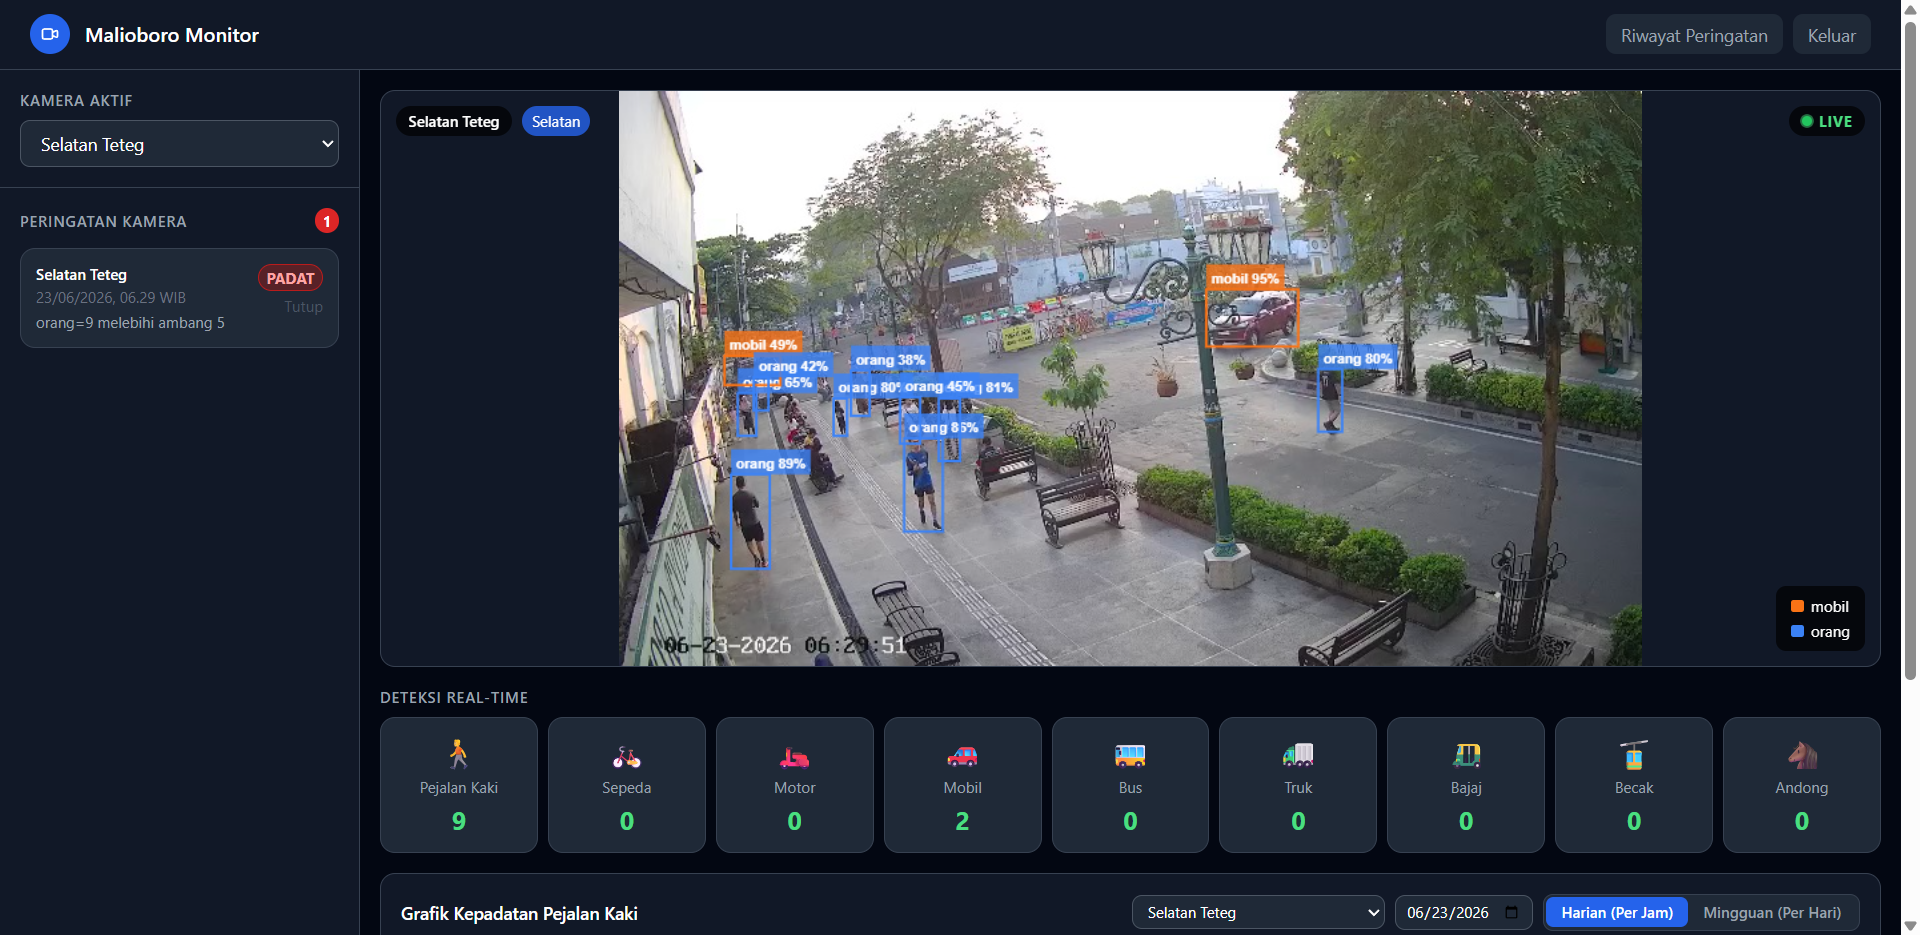
\includegraphics[width=\textwidth]{contents/chapter-4/ss_dasbor.png}
    \caption{Tampilan \textit{dashboard} utama dengan deteksi langsung, panel peringatan kamera, dan ringkasan jumlah objek per kelas.}
    \label{fig:dasbor}
\end{figure}

Gambar \ref{fig:dasbor} memperlihatkan kotak deteksi tergambar di atas \textit{stream} 
video langsung, masing-masing diberi label kelas dan nilai keyakinan, sesuai rancangan pada 
Subbab \ref{sec:sistem}. Panel ringkasan di bagian bawah menunjukkan jumlah deteksi tiap 
kelas pada \textit{frame} saat itu, yaitu sembilan orang dan dua mobil, yang sesuai dengan 
jumlah kotak yang tergambar pada citra. Panel peringatan kamera di sisi kiri menampilkan 
satu notifikasi aktif berstatus padat dengan keterangan "orang=9 melebihi ambang 5", yang 
menunjukkan mekanisme notifikasi yang dirancang pada Subbab \ref{sec:sistem} berhasil 
terpicu sesuai kondisi kepadatan yang terdeteksi.

Nilai ambang 5 pada notifikasi tersebut sengaja diturunkan dari ambang sesungguhnya untuk 
keperluan pengujian, bukan nilai yang dipakai pada operasional sebenarnya. Ambang 
sesungguhnya dihitung dari luas area pejalan kaki yang telah diukur pada Subbab 
\ref{sec:sistem}, yaitu 169~m\textsuperscript{2} untuk kamera seberang Gedung Agung dan 
149~m\textsuperscript{2} untuk kamera Titik Nol, dibagi luas minimum 1,4 
m\textsuperscript{2} per orang pada Standar D. Pembagian ini menghasilkan ambang sekitar 
120 orang untuk kamera seberang Gedung Agung dan 106 orang untuk kamera Titik Nol, dan 
menunggu kepadatan sungguhan mencapai angka tersebut secara alami tidak praktis untuk 
keperluan pengujian fungsional pada penelitian ini. Nilai 5 dipilih sebagai pengganti 
sementara agar notifikasi dapat dipicu dan diverifikasi dalam waktu pengujian yang wajar, 
sedangkan ambang berbasis Standar D yang sesungguhnya, yaitu 120 dan 106 orang, tetap 
menjadi nilai yang diterapkan pada konfigurasi akhir sistem.

\subsection{Hasil Grafik Kepadatan dan Riwayat Peringatan}
\label{sec:hasil_grafik_riwayat}

Grafik kepadatan dan mekanisme riwayat peringatan yang dirancang pada Subbab 
\ref{sec:sistem} diuji untuk memastikan keduanya mencerminkan kondisi kepadatan secara 
akurat dan dapat ditelusuri ulang oleh operator. Pengujian dilakukan dengan mengamati 
kedua komponen tersebut saat sistem berjalan dan menerima deteksi dari kamera secara 
\textit{real-time}. Gambar \ref{fig:grafik_kepadatan} menunjukkan grafik kepadatan harian 
untuk kamera Selatan Teteg pada tanggal pengujian.

\begin{figure}[htbp]
    \centering
    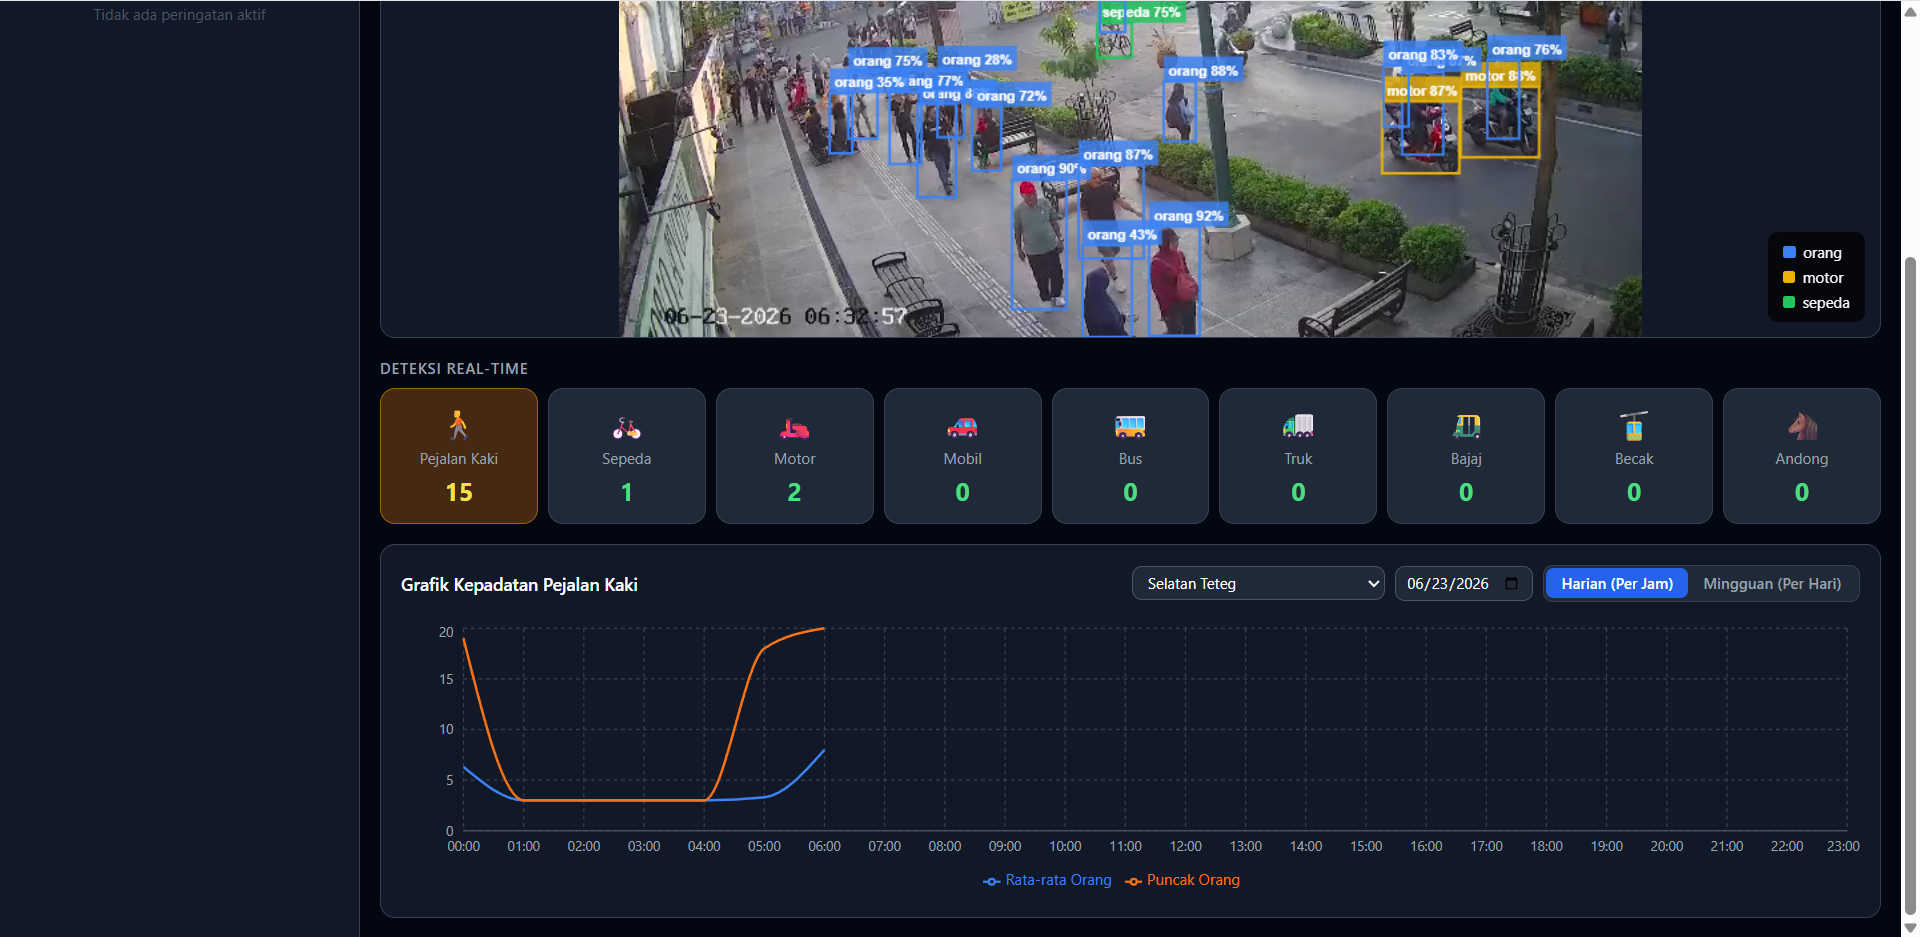
\includegraphics[width=\textwidth]{contents/chapter-4/ss_grafik_kepadatan.png}
    \caption{Grafik kepadatan pejalan kaki harian (per jam) untuk kamera Selatan Teteg, menampilkan rata-rata dan puncak jumlah orang.}
    \label{fig:grafik_kepadatan}
\end{figure}

Gambar \ref{fig:grafik_kepadatan} memperlihatkan dua garis sesuai rancangan pada Subbab 
\ref{sec:sistem}, yaitu rata-rata dan puncak jumlah orang per jam dalam zona waktu WIB. 
Kedua garis menunjukkan pola kepadatan rendah pada dini hari sebelum pukul 04.00 WIB, lalu 
naik tajam menjelang pagi, sesuai dengan karakter kawasan wisata yang ramai pada jam-jam 
aktif. Panel deteksi langsung pada bagian atas gambar yang sama menunjukkan kondisi pukul 
06.32 WIB dengan lima belas orang dan beberapa kendaraan terdeteksi, konsisten dengan tren 
kenaikan yang mulai terlihat pada grafik di jam tersebut.

Riwayat peringatan diuji dengan membuka halaman riwayat dan memeriksa detail salah satu 
peringatan yang tersimpan, sebagaimana ditunjukkan pada Gambar \ref{fig:riwayat_peringatan}. 
Pengujian ini memverifikasi bahwa fitur yang dirancang pada Subbab \ref{sec:sistem}, yaitu 
penyimpanan bukti citra dan kotak deteksi setiap kali peringatan terpicu, benar-benar 
tersimpan dan dapat ditelusuri kembali oleh operator. Detail yang ditampilkan mencakup 
kamera asal, waktu dalam WIB, jenis peringatan, nilai pemicu, dan deskripsi singkat, 
seluruhnya konsisten dengan data yang tercatat pada panel peringatan kamera di Gambar 
\ref{fig:dasbor}.

\begin{figure}[htbp]
    \centering
    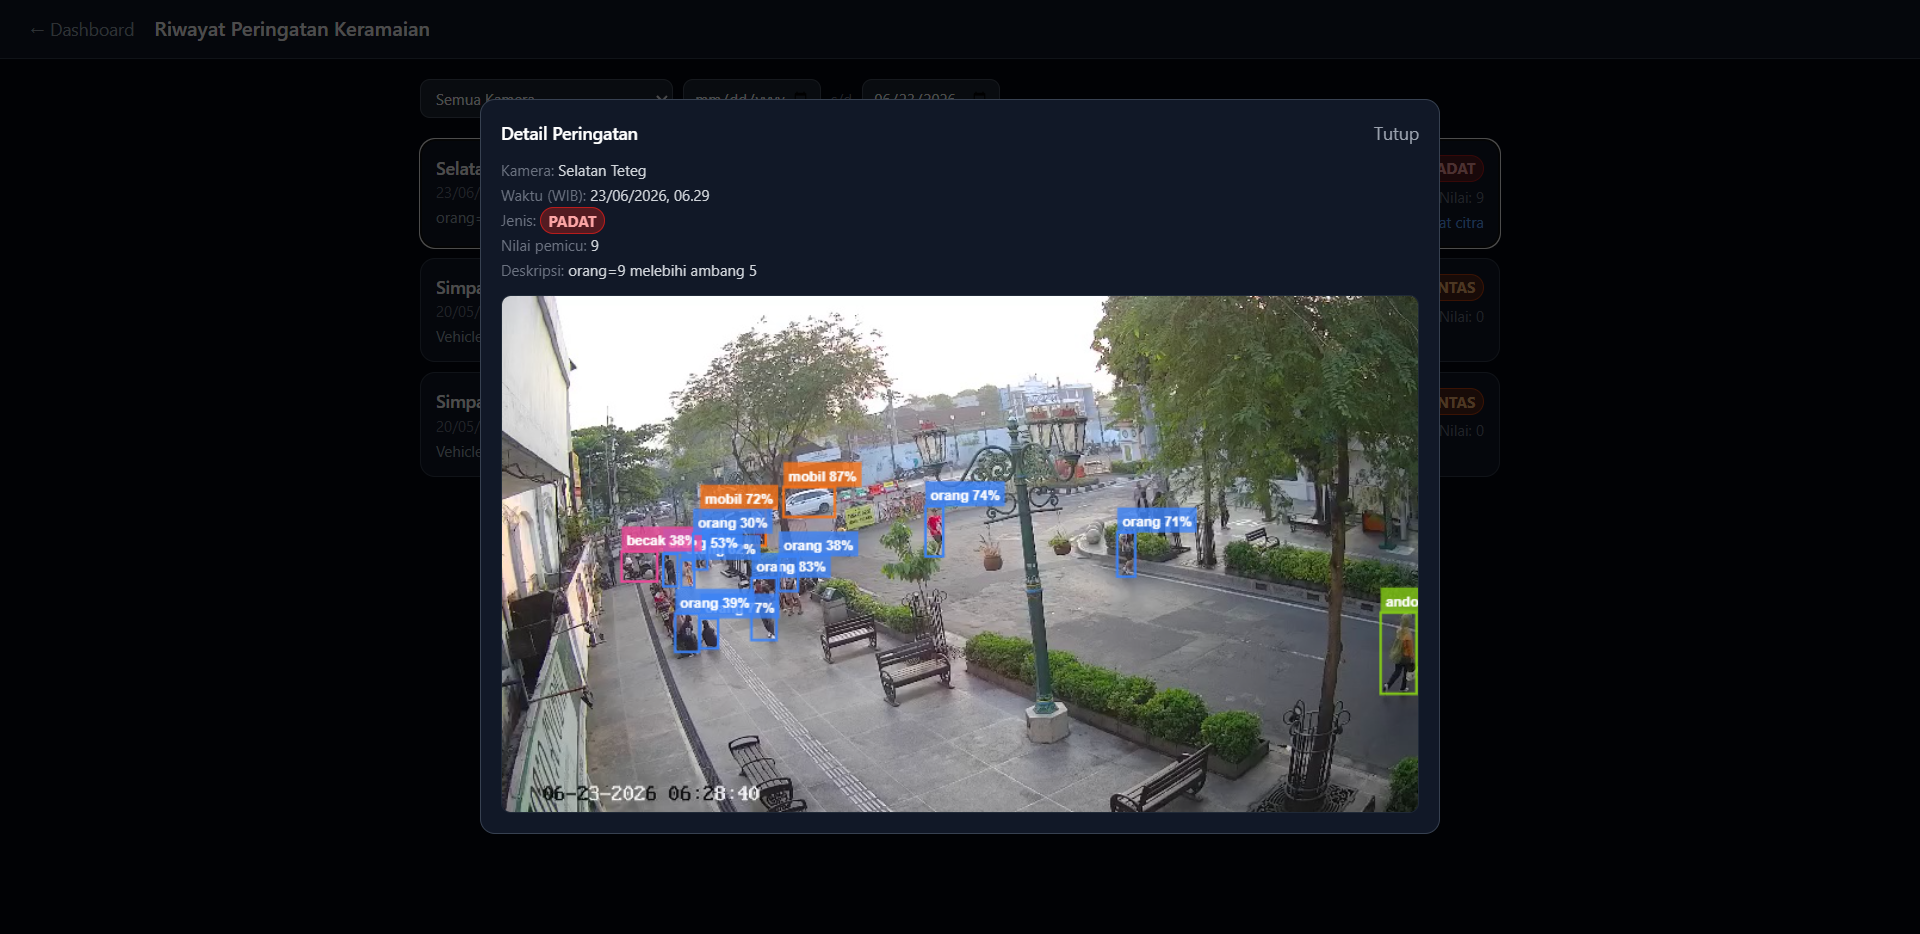
\includegraphics[width=\textwidth]{contents/chapter-4/ss_riwayat_peringatan_keramaian.png}
    \caption{Halaman riwayat peringatan keramaian, menampilkan detail satu peringatan beserta citra CCTV dan kotak deteksinya.}
    \label{fig:riwayat_peringatan}
\end{figure}

Citra pada Gambar \ref{fig:riwayat_peringatan} menunjukkan kotak deteksi tergambar tepat di 
atas citra mentah yang tersimpan, sesuai rancangan pada Subbab \ref{sec:sistem} bahwa citra 
disimpan tanpa anotasi dan kotak deteksi digambar ulang dari data koordinat saat ditampilkan. 
Keberhasilan rekonstruksi kotak deteksi ini pada halaman riwayat membuktikan bahwa 
pendekatan penyimpanan hemat tersebut tidak mengorbankan kelengkapan bukti visual yang dapat 
ditinjau ulang oleh operator. Dengan demikian, ketiga pengujian pada subbab ini, yaitu 
antarmuka deteksi langsung, grafik kepadatan, dan riwayat peringatan, menunjukkan sistem 
berfungsi sesuai rancangan dan berhasil mewujudkan tujuan ketiga penelitian.

\section{Sintesis Temuan}
\label{sec:diskusi_temuan}

Bagian-bagian sebelumnya pada bab ini telah memaparkan hasil secara berurutan mengikuti 
tujuan penelitian, mulai dari pembentukan dataset, perbandingan model, penyetelan, hingga 
implementasi sistem. Subbab ini merangkum keterkaitan antar hasil tersebut, untuk menegaskan 
bagaimana temuan-temuan yang tampak berdiri sendiri pada tiap subbab sesungguhnya saling 
menguatkan satu sama lain. Tiga keterkaitan utama dibahas secara berurutan, yaitu hubungan 
antara pemilihan model dan hasil penyetelan, hubungan antara analisis per kelas sebelum dan 
setelah penyetelan, serta posisi ketidakseimbangan kelas sebagai salah satu faktor yang 
memengaruhi performa, bukan satu-satunya faktor.

Pemilihan yolo11l pada Subbab \ref{sec:pemilihan_model} pada awalnya tidak unggul telak 
dibanding yolov8l, dengan selisih akurasi yang tipis pada metrik longgar. Keputusan ini 
terbukti tepat setelah penyetelan resolusi pada Subbab \ref{sec:hasil_penyetelan}, yang 
mendorong rerata F1 yolo11l dari 0,5962 menjadi 0,6739, melampaui rerata F1 yolov8l pada 
resolusi dasar sebesar 0,6222. Dengan demikian, keunggulan akhir model terpilih bersumber 
dari kombinasi pemilihan arsitektur yang tepat dan optimasi \textit{hyperparameter} yang 
terarah, bukan dari salah satu faktor saja.

Analisis per kelas pada Subbab \ref{sec:hasil_perkelas} dan \ref{sec:hasil_penyetelan_perkelas} 
juga saling menguatkan. Kelemahan model awal pada kelas berukuran kecil seperti sepeda dan 
bajaj, yang teridentifikasi dari \textit{recall} rendah dan diperkuat oleh \textit{confusion 
matrix} pada Subbab \ref{sec:analisis_kurva}, ternyata paling diuntungkan oleh penyetelan 
resolusi. Hubungan ini menunjukkan bahwa strategi penyetelan yang dipilih, yaitu menaikkan 
resolusi masukan, secara tepat menyasar akar permasalahan yang teridentifikasi dari analisis 
sebelumnya, bukan perbaikan yang kebetulan.

Ketidakseimbangan kelas terbukti berpengaruh terhadap performa, tetapi penelitian ini juga 
menemukan bahwa pengaruh tersebut tidak berdiri sendiri. Anomali truk yang berperforma lebih 
baik daripada sepeda meski memiliki \textit{instance} jauh lebih sedikit menunjukkan ukuran 
objek dan kekhasan visual turut memoderasi pengaruh ketidakseimbangan jumlah data. Temuan 
ini melengkapi pemahaman tentang ketidakseimbangan kelas pada deteksi objek multikelas yang 
heterogen secara visual, sebagaimana dibahas pada Subbab \ref{sec:ketidakseimbangan}.

Hasil implementasi pada Subbab \ref{sec:hasil_sistem} melengkapi rangkaian temuan ini 
dengan menunjukkan bahwa pertimbangan ukuran model yang mendasari pemilihan yolo11l pada 
Subbab \ref{sec:pemilihan_model} terbukti relevan di luar sekadar keamanan memori. 
Pengujian kecepatan pada GTX 1650 menunjukkan yolo11l justru lebih cepat dibanding yolov8l 
pada perangkat penerapan, berkebalikan dengan urutan pada GPU V100, sehingga keunggulan 
ukuran yang ringkas memberi manfaat ganda berupa keamanan memori dan kecepatan yang lebih 
baik pada kondisi perangkat terbatas. Pengujian fungsional pada antarmuka, grafik kepadatan, 
dan riwayat peringatan turut menunjukkan bahwa rancangan sistem pada Bab III berhasil 
diwujudkan secara nyata, dengan notifikasi yang terpicu sesuai ambang dan kotak deteksi yang 
berhasil direkonstruksi dari data tersimpan. Secara keseluruhan, ketiga tujuan penelitian 
ini saling terkait erat, yaitu dataset yang terbentuk pada tujuan pertama menjadi dasar 
perbandingan model pada tujuan kedua, dan model yang terpilih serta dioptimasi pada tujuan 
kedua terbukti layak diterapkan pada sistem yang menjawab tujuan ketiga, baik dari sisi 
akurasi maupun kecepatan pada perangkat target.
